\chapter{Inner-Loop Control Design}\label{ch.innerLoop}

This chapter presents a new method of synthesizing an output feedback adaptive controller for a class of uncertain, non-square, multi-input multi-output systems given by\ \eqref{eqn.xdotpunc}.
The main challenge that needs to be addressed is the determination of a corresponding square and strictly positive real transfer function.
This chapter presents a new procedure to synthesize two gain matrices that allows the realization of such a transfer function, thereby allowing a globally stable adaptive output feedback law to be generated.

The unique features of this output feedback adaptive controller are a baseline controller that uses a Luenberger observer, a closed-loop reference model, manipulations of a bilinear matrix inequality, and the Kalman-Yakubovich Lemma.
Using these features, a simple design procedure is proposed for the adaptive controller, and the corresponding stability property is established.
The proposed adaptive controller is compared to the classical multi-input multi-output adaptive controller.

A state feedback linear quadratic regulator (LQR) baseline controller with integral action and augmented with an adaptive component has proven to be an effective choice for accommodating the parametric uncertainties present in flight control applications, and ensuring satisfactory reference tracking\ \cite{crespo.adaptivegtm.2009, dydek.adaptivex15.2010, gibson.adaptive.2008, jang.adaptive.2007, lavretskywise.book.2013, matsutani.adaptivegtm.2009, wiese.adaptive.2013}.
However, such a controller requires that the state is measurable, which may not always be possible.
Also, inaccuracies in the system output measurements may render state feedback controllers sensitive to measurement errors and thus not applicable.
For these reasons there has been an increasing drive to develop an adaptive output feedback extension of the robust integral-augmented LQR baseline plus adaptive controller.

Existing classical methods of multi-input multi-output (MIMO) output feedback adaptive control are applicable for plants that are square\ \cite{tao.multivariable.2014}.
An $m\times m$ transfer matrix is used to represent the dynamic behavior of the plant, and the existence of a stable adaptive solution depends on the available prior information about this plant transfer matrix\ \cite{narendra.stable.2005, singh.prior.1984}.
The solution relies on non-minimal controller representations to dynamically decouple the plant, and the controller structure consists of a feedforward gain and two filters in the feedback path, the order of which depends on $m$ and an upper bound on the observability index of the plant, $\nu$.
The resulting classical MIMO adaptive solution will introduce $2m\nu$ controller states and $2m^{2}\nu$ adjustable parameters.

More recent methods of MIMO output feedback adaptive control have adopted a Luenberger observer-based approach in which a \textit{minimal} observer is used to generate a state estimate to use for feedback control\ \cite{lavretsky.output.2010, lavretskywise.book.2013, qu.jgcd.2016, qu.gnc.2013, wise.obltrdesign.2013}.
This observer also serves as the reference model which is used by the adaptive controller, and the presence of the observer feedback gain $L$ provides the structure known as the closed-loop reference model, or CRM\ \cite{gibson.aiaacrm.2012, gibson.acc.2013, gibson.ecc.2013, gibson.ieeeaccess.2013}.
These CRM based approaches have relied on the so-called squaring-up procedure\ \cite{misra.squareup.1992} to add fictitious inputs to a tall system (one where the dimension of the output is greater than the dimension of the input) making it square and ensuring any transmission zeros are stable.
These fictitious inputs are used only to synthesize a postcompensator $S_{1}$ and the CRM gain $L$ which ultimately render a set of underlying error dynamics strictly positive real (SPR).
These SPR error dynamics allowed stable update laws to be chosen to guarantee system stability.
Note that systems with transmission zeros cannot be squared up using the method as described in Reference\ \cite{misra.squareup.1992}, which has led to a recent modification to overcome this limitation and allow the design of output feedback controllers for systems with stable transmission zeros\ \cite{quwiese.ifac.2014}.
One of the limitations of the existing approaches is in their parameterization of all of the solutions $L$ by just a few scalar parameters which must be picked sufficiently large so as to guarantee stability.
Parameterizing the solutions in this way reduces the degrees of freedom the control designer has, which may limit the robustness of the control design, and require larger gains than otherwise might be necessary.

The CRM based output feedback design procedure proposed in this paper takes an alternative approach to synthesizing $S_{1}$ and $L$ which does not require the system first be squared-up.
Instead, the postcompensator $S_{1}$ is determined as a generalized inverse of the system matrices, and a state feedback approach is used to stabilize a related lower order plant subsystem.
This results in a feasible linear matrix inequality (LMI) which is solved to yield $L$.
This LMI is the same inequality which is solved in the existing approaches, and depends on a positive definite matrix $P_{x}$.
In the existing approaches, this matrix is parameterized by a single scalar parameter; the proposed approach provides the set of all $P_{x}$ which admit solutions $L$ to the inequality, in terms of a symmetric $(n-m)\times(n-m)$ matrix $X$.
Once this $P_{x}$ is obtained the, proposed approach then guarantees the existence of a solution $L$ to the LMI, which again provides many degrees of freedom, beyond the scalar parameter used to parameterize the solutions in the existing approaches.
While the proposed approach does not provide a closed-form solution to the matrix $L$, it is the degrees of freedom in the matrix $X$ and the solution to the LMI which can be leveraged to yield improved control designs.

In this thesis the case of tall systems is considered, but the case of wide systems holds by duality.
Furthermore, because $L$ is a component of both the baseline and adaptive controllers, it is crucial that it be selected to provide good frequency domain properties for the baseline control system, as well as desirable adaptive control performance.
This procedure is able to exploit the structure of the given system to obtain a large amount of freedom in the selection of $L$ in order to achieve a robust baseline control design and the desired adaptive performance.

In Section~\ref{sec.controlproblem} the control architecture is presented, and the control problem of interest formulated using this proposed architecture.
Section~\ref{sec.adaptivecontroldesign} provides a constructive procedure for obtaining an update law for an adaptive controller which guarantees global stability.
Section~\ref{sec.AdaptiveComparison} compares the proposed controller to the existing classical controller, Section~\ref{sec.innerLoopNumericalExample} provides some numerical examples applying the controller to several systems, and Section~\ref{sec.innerLoopConclusion} provides some concluding remarks about the inner-loop controller developed in this chapter.

\section{Inner-loop Control Problem Formulation}\label{sec.controlproblem}

For the design of the inner-loop controller, consider systems of the form\ \eqref{eqn.xdotpunc}.
The \textit{control goal} is to design the input $u(t)$ which will make $z_{p}(t)$ track the command $z_{p,\text{cmd}}(t)$ with bounded errors in the presence of the uncertainties $\Lambda$ and $\Psi_{p}$.
Make the following assumptions about the system in\ \eqref{eqn.innerLoopDynamicsUncertain}.

\begin{customthm}{1} $\;$\label{ass.plant}
  \begin{enumerate}[\Alph{enumi}), ref=\Alph{enumi}] % chktex 9 chktex 10
    \itemsep0em
    \item{$(A_{p},B_{p})$ is controllable.\label{ass.p.cont}}
    \item{$(A_{p},C_{p})$ is observable.\label{ass.p.obsv}}
    \item{$B_{p}$, $C_{p}$, and $C_{p}B_{p}$ are full rank.\label{ass.p.rank}}
    \item{Any finite transmission zeros of $(A_{p},B_{p},C_{p},0)$ are strictly stable, and the rank of the following matrix is full\label{ass.p.tzero}}
    \begin{equation*}
      \text{rank}\left(
      \begin{bmatrix}
        A_{p} & B_{p} \\
        C_{pz} & D_{pz}
      \end{bmatrix}\right)
      =n_{p}+n_{e}
    \end{equation*}
    \item{%
      \begin{enumerate}[(\alph{enumii}), ref=\alph{enumii}]
        \item{$\Lambda$ is nonsingular and diagonal with entries of known sign\label{ass.p.unc.lambda}}
        \item{$\|\Psi_{p}\|_{2}<\Psi_{\rm{\max}}<\infty$, where $\Psi_{\rm{\max}}$ is known\label{ass.p.unc.wp}}
      \end{enumerate}\label{ass.p.unc}
    }
  \end{enumerate}
\end{customthm}

In order to facilitate command tracking, integral action is introduced, and for this purpose an additional state $x_e$ is defined as
\begin{equation}
  \label{eqn.xedot}
  \dot{x}_{e}(t) = z_{p,\text{cmd}}(t) - z_{p}(t)
\end{equation}
This integral error state is appended to the plant in\ \eqref{eqn.innerLoopDynamicsUncertain} leading to the following integral-augmented open-loop dynamics
\begin{equation}
  \label{eqn.uncsystemfull}
  \begin{split}
    \begin{bmatrix}
      \dot{x}_{p}(t) \\
      \dot{x}_{e}(t)
    \end{bmatrix}
    &=
    \begin{bmatrix}
      A_{p} & 0 \\
      -C_{pz} & 0
    \end{bmatrix}
    \begin{bmatrix}
      x_{p}(t) \\
      x_{e}(t)
    \end{bmatrix}
    +
    \begin{bmatrix}
      B_{p} \\
      -D_{pz}
    \end{bmatrix}\bigr(\Lambda u(t)+\Psi_{p}^{\top}x_{p}(t)\bigr)
    +
    \begin{bmatrix}
      0 \\
      I
    \end{bmatrix}z_{p,\text{cmd}}(t) \\
    \begin{bmatrix}
      y_{p}(t) \\
      x_{e}(t)
    \end{bmatrix}
    &=
    \begin{bmatrix}
      C_{p} & 0 \\
      0 & I
    \end{bmatrix}
    \begin{bmatrix}
      x_{p}(t) \\
      x_{e}(t)
    \end{bmatrix} \\
    z_{p}(t)
    &=
    \begin{bmatrix}
      C_{pz} & 0
    \end{bmatrix}
    \begin{bmatrix}
      x_{p}(t) \\
      x_{e}(t)
    \end{bmatrix}
    +
    D_{pz}\bigr(\Lambda u(t) + \Psi_{p}^{\top}x_{p}(t)\bigr)
  \end{split}
\end{equation}
Define the unknown matrix $\Psi$ as
\begin{equation*}
  \Psi=
  [\begin{array}{cc} {\Psi_{p}}^{\top} & 0_{m\times n_{e}} \end{array}]^{\top}
\end{equation*}
Eq.\ \eqref{eqn.uncsystemfull} can then be expressed as
\begin{equation}
  \label{eqn.uncertainss}
  \begin{split}
    \begin{bmatrix}
      \dot{x}_{p}(t) \\
      \dot{x}_{e}(t)
    \end{bmatrix}
    &=
    \begin{bmatrix}
      A_{p} & 0 \\
      -C_{pz} & 0
    \end{bmatrix}
    \begin{bmatrix}
      x_{p}(t) \\
      x_{e}(t)
    \end{bmatrix}+
    \begin{bmatrix}
      B_{p} \\
      -D_{pz}
    \end{bmatrix}\Psi^{\top}
    \begin{bmatrix}
      x_{p}(t) \\
      x_{e}(t)
    \end{bmatrix}+
    \begin{bmatrix}
      B_{p} \\
      -D_{pz}
    \end{bmatrix}\Lambda u(t) +
    \begin{bmatrix}
      0 \\
      I
    \end{bmatrix}z_{p,\text{cmd}}(t) \\
    \begin{bmatrix}
      y_{p}(t) \\
      x_{e}(t)
    \end{bmatrix}
    &=
    \begin{bmatrix}
      C_{p} & 0 \\
      0 & I
    \end{bmatrix}
    \begin{bmatrix}
      x_{p}(t) \\
      x_{e}(t)
    \end{bmatrix} \\
    z_{p}(t)
    &=
    \begin{bmatrix}
      C_{pz} & 0
    \end{bmatrix}
    \begin{bmatrix}
      x_{p}(t) \\
      x_{e}(t)
    \end{bmatrix}
    +
    D_{pz}\left(\Lambda u(t) + \Psi^{\top}
    \begin{bmatrix}
      x_{p}(t) \\
      x_{e}(t)
    \end{bmatrix}
    \right)
  \end{split}
\end{equation}
The system in\ \eqref{eqn.uncertainss} can be written more compactly as follows
\begin{equation}
  \label{eqn.uncsystem}
  \begin{split}
    \dot{x}(t) &= Ax(t)+B\bigr(\Lambda u(t)+\Psi^{\top}x(t)\bigr)+B_{\text{cmd}}z_{p,\text{cmd}}(t) \\
    y(t) &= Cx(t) \\
    z_{p}(t) &= C_{z}x(t) + D_{pz}\bigr(\Lambda u(t)+\Psi^{\top}x(t)\bigr)
  \end{split}
\end{equation}
where $A\in\mathbb{R}^{n\times n}$, $B\in\mathbb{R}^{n\times m}$, $B_{\text{cmd}}\in\mathbb{R}^{n\times n_{e}}$, and $C\in\mathbb{R}^{p\times n}$ are the known matrices given by
\begin{equation*}
  \begin{gathered}
    A=
    \begin{bmatrix}
      A_{p} & 0_{n_{p}\times n_{e}} \\
      -C_{pz} & 0_{n_{e}\times n_{e}}
    \end{bmatrix} \quad
    B=
    \begin{bmatrix}
      B_{p} \\
      -D_{pz}
    \end{bmatrix}
    \quad
    B_{\text{cmd}}=
    \begin{bmatrix}
      0_{n_{p}\times m} \\
      I_{n_{e}\times n_{e}}
    \end{bmatrix}
    \quad
    C=
    \begin{bmatrix}
      C_{p} & 0_{\ell\times n_{e}} \\
      0_{n_{e}\times n_{p}} & I_{n_{e}\times n_{e}}
    \end{bmatrix} \\
    C_{z} =
    \begin{bmatrix}
      C_{pz} & 0
    \end{bmatrix}
  \end{gathered}
\end{equation*}
Note that $p=\ell+n_{e}$.
It can be shown that Assumption~\ref{ass.plant} regarding the plant in\ \eqref{eqn.xdotpunc} is equivalent to Assumption~\ref{ass.uncsystem} regarding the system $(A,B,C,0)$ in\ \eqref{eqn.uncsystem}, which is stated below.

\begin{customthm}{$1^{\prime}$} $\;$\label{ass.uncsystem}
  \begin{enumerate}[\Alph{enumi}), ref=\Alph{enumi}] % chktex 9 chktex 10
    \itemsep0em
    \item{$(A,B)$ is controllable.\label{ass.cont}}
    \item{$(A,C)$ is observable.\label{ass.obsv}}
    \item{$B$, $C$, and $CB$ are full rank.\label{ass.rank}}
    \item{Any finite transmission zeros of $(A,B,C,0)$ are strictly stable.\label{ass.tzero}}
    \item{%
      \begin{enumerate}[(\alph{enumii}), ref=\alph{enumii}]
        \item{$\Lambda$ is nonsingular and diagonal with entries of known sign\label{ass.unc.lambda}}
        \item{$\|\Psi\|_{2}<\Psi_{\rm{\max}}<\infty$, where $\Psi_{\rm{\max}}$ is known\label{ass.unc.w}}
      \end{enumerate}\label{ass.unc}
    }
    \item{$(A,B,C,0)$ is tall: $p>m$.\label{ass.tall}}
  \end{enumerate}
\end{customthm}

\begin{rem-dan}
  The system in\ \eqref{eqn.xdotpunc} satisfying Assumption~\ref{ass.plant}\ref{ass.p.cont}-\ref{ass.p.tzero} when augmented with the integral error state as shown in\ \eqref{eqn.uncsystemfull} also satisfies Assumption~\ref{ass.uncsystem}\ref{ass.cont}-\ref{ass.tzero}.
  In other words, under Assumption~\ref{ass.plant}\ref{ass.p.cont}-\ref{ass.p.tzero}, integral error augmentation does not destroy controllability, observability, or the rank conditions.
  Nor does it add any transmission zeros\ \cite{lavretsky.output.2010}.
\end{rem-dan}

\begin{rem-dan}
  Assumptions~\ref{ass.uncsystem}\ref{ass.cont} and~\ref{ass.uncsystem}\ref{ass.obsv} are standard.
  Assumption~\ref{ass.uncsystem}\ref{ass.rank} implies that inputs and outputs are not redundant, as well as a MIMO equivalent of relative degree unity.
  Assumption~\ref{ass.uncsystem}\ref{ass.tzero} is a standard requirement for output feedback adaptive control.
  Assumption~\ref{ass.uncsystem}\ref{ass.tall} can be considered without loss of generality as the case of wide systems $p<m$ holds by duality.
  The case of square systems has been given in Reference\ \cite{huang.designspr.1999} and is discussed in Section~\ref{sec.adaptivecontroldesign}.
\end{rem-dan}

\subsection{Baseline Control Design}

The underlying problem here is to design a control input $u(t)$ in\ \eqref{eqn.uncsystem} so that the closed-loop system has bounded solutions and $z_{p}(t)$ tends to  $z_{p,\text{cmd}}(t)$ with bounded errors in the presence of the uncertainties $\Lambda$ and $\Psi$.
In this section, the baseline control design for the nominal case when there are no uncertainties present, that is when $\Lambda=I$ and $\Psi=0$, is described.

A controller along the lines of References\ \cite{lavretsky.output.2010, qu.gnc.2013, wise.obltrdesign.2013} is proposed, as it leads to a low order robust controller.
This controller includes a Luenberger observer together with LQR feedback control gains.
As the ultimate goal is to develop an adaptive controller which in turn requires a reference model, a control design where the reference model has components of an observer as well, is proposed.
In particular, a feedback component is introduced into the reference model, with the corresponding feedback gain $L$ chosen similar to a Luenberger gain, that is, so that it ensures adequate stability margins for the nominal closed-loop system.
The resulting reference model is referred to as a closed-loop reference model (CRM) which has been shown recently to result in highly desirable transient properties\ \cite{gibson.aiaacrm.2012,gibson.ecc.2013,gibson.ieeeaccess.2013,gibson.acc.2013}.
To obtain the reference model, consider\ \eqref{eqn.uncertainss} with no uncertainty, that is $\Lambda=I$ and $\Psi=0$, with a reference input $r(t)$ in place of $z_{p,\text{cmd}}(t)$, and the addition of the CRM gain $L$.
The reference model state $x_{m}(t)$ is used in place of the plant state $x(t)$, and a baseline control input $u_{\text{bl}}(t)$ in place of the control input $u(t)$.
\begin{equation}
  \label{eqn.uncertainssRefModel}
  \begin{split}
    \begin{bmatrix}
      \dot{x}_{pm}(t) \\
      \dot{x}_{em}(t)
    \end{bmatrix}
    &=
    \begin{bmatrix}
      A_{p} & 0 \\
      -C_{pz} & 0
    \end{bmatrix}
    \begin{bmatrix}
      x_{pm}(t) \\
      x_{em}(t)
    \end{bmatrix} +
    \begin{bmatrix}
      B_{p} \\
      -D_{pz}
    \end{bmatrix} u_{\text{bl}}(t) +
    \begin{bmatrix}
      0 \\
      I
    \end{bmatrix}r(t)
    +
    \begin{bmatrix}
      L_{p} \\
      L_{e}
    \end{bmatrix}(y_{m}(t)-y(t)) \\
    \begin{bmatrix}
      y_{pm}(t) \\
      x_{em}(t)
    \end{bmatrix}
    &=
    \begin{bmatrix}
      C_{p} & 0 \\
      0 & I
    \end{bmatrix}
    \begin{bmatrix}
      x_{pm}(t) \\
      x_{em}(t)
    \end{bmatrix} \\
    z_{pm}(t)
    &=
    \begin{bmatrix}
      C_{pz} & 0
    \end{bmatrix}
    \begin{bmatrix}
      x_{pm}(t) \\
      x_{em}(t)
    \end{bmatrix}
    +
    D_{pz}u_{\text{bl}}(t)
  \end{split}
\end{equation}
The reference model\ \eqref{eqn.uncertainssRefModel} can be written more compactly as
\begin{equation}
  \label{eqn.refmodel0}
  \begin{split}
    \dot{x}_{m}(t) &= Ax_{m}(t) + Bu_{\text{bl}}(t) + B_{\text{cmd}}r(t) + L\bigr(y_{m}(t)-y(t)\bigr) \\
    y_{m}(t) &= Cx_{m}(t) \\
    z_{pm}(t) &= C_{z}x_{m}(t) + D_{pz}u_{\text{bl}}(t)
  \end{split}
\end{equation}
where
\begin{equation*}
  L =
  \begin{bmatrix}
    L_{p} \\
    L_{e}
  \end{bmatrix}
\end{equation*}
Propose the following baseline controller that can guarantee command tracking and a certain amount of stability margins for the nominal closed-loop system.
That is, propose the following form of the baseline control law which will be used to construct the reference model in\ \eqref{eqn.refmodel0}
\begin{equation}
  \label{eqn.ubl}
  u_{\text{bl}}(t) = K_{x}^{\top}x_{m}(t)
\end{equation}
where $K_{x}$ is chosen such that $A_{m}=A+BK_{x}^{\top}$ is Hurwitz.
In addition, $K_{x}$ should be selected to provide the desired closed-loop performance of the nominal system.
With such a $K_{x}$, and baseline control law, the reference model in\ \eqref{eqn.refmodel0} becomes
\begin{equation}
  \label{eqn.refmodel}
  \begin{split}
    \dot{x}_{m}(t) &= A_{m}x_{m}(t) + B_{\text{cmd}}r(t) + L\bigr(y_{m}(t)-y(t)\bigr) \\
    y_{m}(t) &= Cx_{m}(t) \\
    z_{pm}(t) &= C_{z}x_{m}(t) + D_{pz}K_{x}^{\top}x_{m}(t)
  \end{split}
\end{equation}
With the reference model constructed using the nominal system, that is\ \eqref{eqn.uncsystem} with $\Lambda=I$ and $\Psi=0$, which contains integral action, guarantees that $z_{pm}(t)$ will track $z_{p,\text{cmd}}(t)$ with bounded errors.
Essentially the reference model serves as a command pre-filter, so that $z_{pm}(t)$ is just a filtered version of $z_{p,\text{cmd}}(t)$.

The block diagram for the baseline controller is depicted in Figure~\ref{fig.innerLoopBaseline}.
As discussed above, while the selection of $L$ is done so as to allow the use of an adaptive law, it should also provide sufficient stability margins for the baseline system.
This baseline control architecture is simply a classical dynamic output feedback compensator with a closed-loop Luenberger state estimator.

\begin{figure}[H]
  \begin{center}
    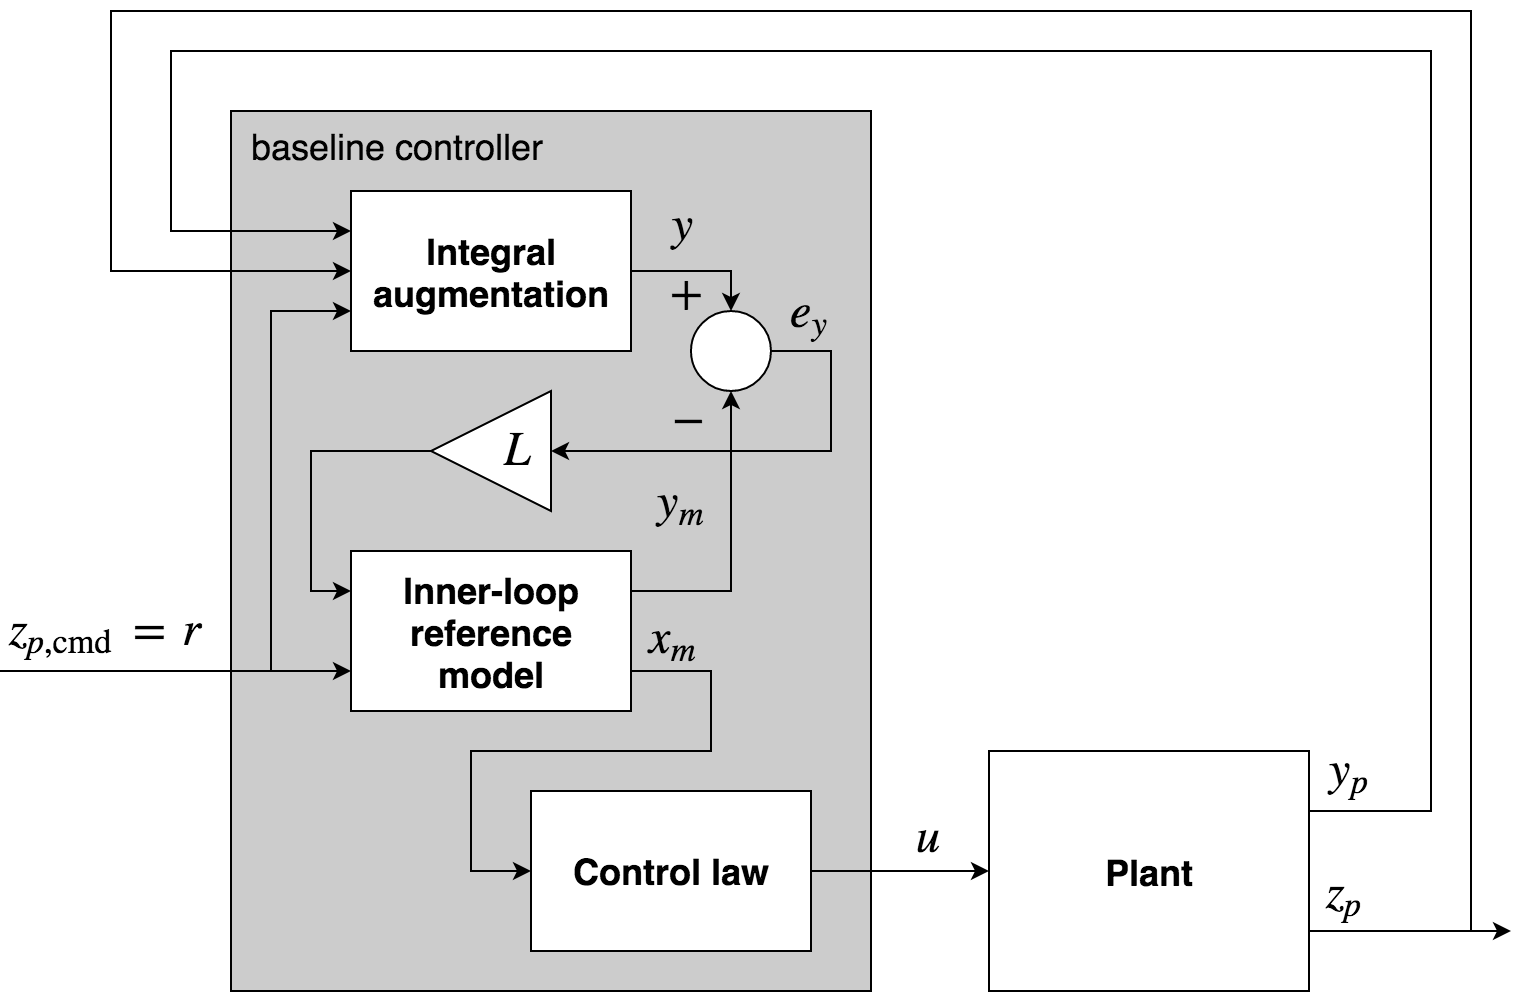
\includegraphics[width=6.5in]{\figurepath/innerLoopBaseline.png}
    \vspace{-0.1in}
    \caption{Inner-loop baseline control block diagram.\label{fig.innerLoopBaseline}}
  \end{center}
\end{figure}

\subsection{Adaptive Controller}

With the baseline controller determined as above, the next step is to design an adaptive controller in the presence of $\Lambda\neq I$ and $\Psi\neq 0$.
Suppose the nominal controller in\ \eqref{eqn.ubl} is augmented with an adaptive element as
\begin{equation}
  \label{eqn.u}
  u(t) = \bigr(K_{x}(t)+\Theta(t)\bigr)^{\top}x_{m}(t)
\end{equation}
where $\Theta(t)$ is to be determined by a suitable update law.
The question is if the introduction of the parameter $\Theta(t)$ as in\ \eqref{eqn.u} is sufficient to accommodate the parametric uncertainties.
For this purpose, a matching condition as described in Remark~\ref{rem.matching}, is introduced below.

\begin{rem-dan}[(Matching condition)]\label{rem.matching}
  The selection of the reference model state matrix as $A_{m}=A+BK_{x}^{\top}$ guarantees the existence of a parameter $\Theta^{*}$ that satisfies the following matching condition.
  \begin{equation*}
    A_{m}=A+B\Psi^{\top}+B\Lambda\bigr(\Theta^{*\top}+K_{x}^{\top}\bigr)
  \end{equation*}
  where $\Theta^{*}$ is given by
  \begin{equation*}
    \Theta^{*\top}=(\Lambda^{-1}-I)K_{x}^{\top}-\Psi^{\top}
  \end{equation*}
\end{rem-dan}

Given a system satisfying Assumption~\ref{ass.uncsystem}, the matching condition in Remark~\ref{rem.matching}, and the proposed control architecture, the reference tracking control problem is reduced to selecting the CRM gain $L$ in\ \eqref{eqn.refmodel} and a suitable adaptive law for updating $\Theta(t)$ in\ \eqref{eqn.u}.

In summary, the problem that is addressed in this chapter is the determination of an adaptive augmented robust baseline output feedback controller as in\ \eqref{eqn.u} to control the plant in\ \eqref{eqn.uncsystem} using the CRM/Observer as in\ \eqref{eqn.refmodel}.
This in turn necessitates finding an adaptive law for adjusting $\Theta$ in\ \eqref{eqn.u} and the observer gain $L$ in\ \eqref{eqn.refmodel}.
The main tools used for determining the adaptive controller were provided in Appendix~\ref{app.preliminaries} and involve the Kalman-Yakubovich\ \cite{narendra.stable.2005} and matrix elimination lemmas\ \cite{boyd.lmibook.1994}, which help reduce the problem of finding $L$ to a state feedback problem of a related lower order subsystem.
The complete adaptive control design and the corresponding stability result are presented in Section~\ref{sec.adaptivecontroldesign}.

\section{Adaptive Control Design}\label{sec.adaptivecontroldesign}

In this section the process for selecting the CRM gain $L$ in\ \eqref{eqn.refmodel} and the update law for $\Theta(t)$ in\ \eqref{eqn.u} is provided.
To accomplish the goal of reference tracking an approach which focuses on the error between the closed-loop plant and the reference model states, as opposed to each of these trajectories individually, is taken.
Thus, the goal of reference tracking can be ensured by appropriately selecting the update law to drive this state error to zero.
Similarly, consider the error between the parameter $\Theta(t)$ in\ \eqref{eqn.u} and $\Theta^{*}$ in Remark~\ref{rem.matching}.
The resulting state tracking error and parameter error, respectively, can be defined as
\begin{align*}
  e_{x}(t) &= x(t) - x_{m}(t) \\
  \widetilde{\Theta}(t) &= \Theta(t) - \Theta^{*}
\end{align*}
The problem of finding an adaptive law for $\Theta(t)$ that guarantees stability depends on the relationship between the two errors above.
This relation, denoted as \textit{error model}, in turn provides cues for determining the adaptive law.
In the problem under consideration, the underlying error model can be described as
\begin{equation}
  \label{eqn.errordynamics1}
  \begin{split}
    \dot{e}_{x}(t) &= (A+LC+B\Psi^{\top})e_{x}(t) + B\Lambda\widetilde{\Theta}^{\top}x_{m}(t) + B_{\text{cmd}}\bigr(z_{p,\text{cmd}}(t) - r(t)\bigr) \\
    e_{y}(t) &= Ce_{x}(t) \\
  \end{split}
\end{equation}
where $e_{y}(t)$ is the measured output error.
Furthermore, select the reference model input $r(t)$ as
\begin{equation}
  \label{eqn.zcmd1}
  r(t) = z_{p,\text{cmd}}(t)
\end{equation}
which is typical in adaptive control and further simplifies the error dynamics in\ \eqref{eqn.errordynamics1} to
\begin{equation}
  \label{eqn.errordynamics2}
  \begin{split}
    \dot{e}_{x}(t) &= \bigr(A+LC+B\Psi^{\top}\bigr)e_{x}(t) + B\Lambda\widetilde{\Theta}^{\top}(t)x_{m}(t) \\
    e_{y}(t) &= Ce_{x}(t) \\
  \end{split}
\end{equation}
As mentioned earlier, the problem of finding a stabilizing adaptive controller is equivalent to finding an $L$ and an adaptive law for adjusting $\widetilde{\Theta}(t)$ in\ \eqref{eqn.errordynamics2}.
Determining a stable adaptive law for an error model as in\ \eqref{eqn.errordynamics2} relies on properties of an underlying transfer function that is SPR\ \cite{narendra.stable.2005}, which in turn enables the use of  Lemma 1 in Appendix~\ref{app.preliminaries}.
However, the definition of SPR is restricted to square transfer functions.
As such, for these properties to be applicable to the error model in\ \eqref{eqn.errordynamics2}, a suitable static postcompensator $S_1\in\mathbb{R}^{m\times p}$ has to be chosen such that
\begin{equation*}
  S_{1}C(sI-A-LC-B\Psi^{\top})^{-1}B \in\mathbb{R}_{p}^{m\times m}(s)
\end{equation*}
where $\mathbb{R}_{p}(s)$ denotes the ring of \textit{proper} rational transfer functions with coefficients in $\mathbb{R}$.
That is the underlying transfer matrix is square, and therefore can be evaluated in terms of SPR properties.
It is therefore necessary to introduce a synthetic output error $e_{s}(t)$ as
\begin{equation}
  \label{eqn.syntheticoutputerror}
  e_{s}(t) = S_{1}Ce_{x}(t)
\end{equation}
Using the synthetic output error in\ \label{eqn.syntheticoutputerror} in place of the output error, the underlying error model in\ \eqref{eqn.errordynamics2} is modified as
\begin{equation}
  \label{eqn.uncerrdyn}
  \begin{split}
    \dot{e}_{x}(t) &= \bigr(A+LC+B\Psi^{\top}\bigr)e_{x}(t) + B\Lambda\widetilde{\Theta}^{\top}(t)x_{m}(t) \\
    e_{s}(t) &= S_{1}Ce_{x}(t)
  \end{split}
\end{equation}
Thus, the design of an output feedback adaptive controller is reduced to selecting matrices $S_{1}\in\mathbb{R}^{m\times p}$ and $L\in\mathbb{R}^{n\times p}$ such that the error dynamics in\ \eqref{eqn.uncerrdyn} are SPR.\@

In Section~\ref{sec.findingS1andL} a procedure to construct $S_{1}$ and $L$ is provided.
This procedure requires $S_{1}$ to be solved as a generalized inverse based on the matrices of $(A,B,C,0)$ in\ \eqref{eqn.uncsystem} alone.
$L$ is found by satisfying Lemma~\ref{lem.KY} (Kalman-Yakubovich), the solution of which is reduced to a state-feedback problem of a lower-order plant subsystem which ultimately leads to a feasible LMI which is solved numerically to obtain $L$.

\subsection{Finding $S_{1}$ and $L$}\label{sec.findingS1andL}

In this section a method for selecting $S_{1}$ and $L$ which ensure the system in\ \eqref{eqn.uncerrdyn} is SPR, is provided.
The conditions from Lemma~\ref{lem.KY} to ensure $(A+LC+B\Psi^{\top},B,S_{1}C)$ is SPR are given by
\begin{align}
  \label{eqn.lyapal}
  (A+LC+B\Psi^{\top})^{\top}P_{x}+P_{x}(A+LC+B\Psi^{\top}) &< 0 \\
  \label{eqn.S1CB}
  P_{x}B &= (S_{1}C)^{\top}
\end{align}
where, by the corollary to Lemma~\ref{lem.KY} in Appendix~\ref{app.preliminaries}, a $P_{x}$ exists which satisfies\ \eqref{eqn.S1CB} if and only if $S_{1}CB=(S_{1}CB)^{\top}$.

\subsubsection{Finding $S_{1}$}

The matrix $S_{1}$ satisfying\ \eqref{eqn.S1CB} can be computed as a generalized left inverse of $CB$ as
\begin{equation}
  \label{eqn.S1}
  S_{1}=\bigr((CB)^{\top}CB\bigr)^{-1}(CB)^{\top}
\end{equation}
Note that this choice of $S_{1}$ is not unique.
An alternative choice for $S_{1}$ is
\begin{equation}
  \label{eqn.S1alternative}
  S_{1} = B^{\top}C^{\top}K_{s}
\end{equation}
where $K_{s}=K_{s}^{\top}\in\mathbb{R}^{p\times p}$.

% TODO@dpwiese - use \texorpdfstring{$L$}{L}
\subsubsection{Finding $L$}\label{subsection.obtainX}

The annihilator matrices $B^{\perp}$ and $C^{\top\perp}$ in Appendix~\ref{app.preliminaries} are not unique.
In the following subsection the notation $N$ and $M$ is used to represent particular annihilators that satisfy
\begin{equation}
  \label{eqn.NB0CM0}
  NB=0
  \qquad
  CM=0
\end{equation}
as well a few additional desired properties.
That is, $N$ represents a particular $B^{\perp\top}$ and $M$ a particular $C^{\top\perp}$.
Given arbitrary annihilators $B^{\perp}$ and $C^{\top\perp}$ a constructive process for obtaining $N$ and $M$ is provided, and these matrices are then used to find $L$.
The inequality\ \eqref{eqn.lyapal} is satisfied if the following inequality is satisfied
\begin{equation}
  \label{eqn.lyapalQ}
  (A+LC)^{\top}P_{x}+P_{x}(A+LC)+Q_{x}<0
\end{equation}
for
\begin{equation}
  \label{eqn.WBTP}
  \Psi B^{\top}P_{x}+P_{x}B\Psi^{\top}<Q_{x}
\end{equation}
Using\ \eqref{eqn.S1CB}, the inequality\ \eqref{eqn.WBTP} can be written as
\begin{equation}
  \label{eqn.WS1C}
  \Psi S_{1}C+(\Psi S_{1}C)^{\top}<Q_{x}
\end{equation}
Note that $Q_{x}$ satisfying\ \eqref{eqn.WS1C} is independent of $P_{x}$.
Using Lemma~\ref{lem.elimination} in Appendix~\ref{app.preliminaries}, an $L$ exists which satisfies\ \eqref{eqn.lyapalQ} if and only if a $P_{x}$ exists which satisfies
\begin{equation}
  \label{eqn.MAPPAM}
  M^{\top}(A^{\top}P_{x}+P_{x}A)M<-M^{\top}Q_{x}M
\end{equation}
Using\ \eqref{eqn.Psolutions}, $P_{x}$ is given by
\begin{equation}
  \label{eqn.Px}
  P_{x} = (S_{1}C)^{\top}(S_{1}CB)^{-\top}S_{1}C+N^{\top}XN
\end{equation}
Substituting the expression for $P_{x}$ from\ \eqref{eqn.Px} into the inequality\eqref{eqn.MAPPAM} the following is obtained
\begin{equation}
  \label{eqn.NAMlyap}
  (NAM)^{\top}XNM+(NM)^{\top}X(NAM)<-M^{\top}Q_{x}M
\end{equation}
Thus, the problem of finding an SPR $L$ which satisfies the inequality\ \eqref{eqn.lyapal} is now reduced to finding the matrix $X$ satisfying the inequality\ \eqref{eqn.NAMlyap}.
An $X$ satisfying\ \eqref{eqn.NAMlyap} specifies a $P_{x}$ as given in\ \eqref{eqn.Px} that reduces\ \eqref{eqn.lyapal} to a feasible LMI in $L$.
This LMI can then be easily solved using any widely available numerical LMI solver to obtain $L$.

Reference\ \cite{huang.designspr.1999} gave the inequality\ \eqref{eqn.NAMlyap} for a square system, suggesting that $X$ be obtained by solving this LMI numerically.
However, it was shown in Reference\ \cite{kouvaritakis.part1.1976} that for a square system, the eigenvalues of $NAM$ in\ \eqref{eqn.NAMlyap} are the transmission zeros of the system and the annihilators $N$ and $M$ in\ \eqref{eqn.NAMlyap} can be always be selected such that $NM=I$.
Given a square system with only stable transmission zeros, this selection reduces\ \eqref{eqn.NAMlyap} to a Lyapunov equation where the matrix $NAM$ is stable, and the existence of $X>0$ satisfying this inequality is guaranteed\ \cite{barkana.comments.2004}.
Thus, when the system $(A,B,C,0)$ in\ \eqref{eqn.uncsystem} is square, the inequality\ \eqref{eqn.NAMlyap} can be solved to obtain $X$, and $P_{x}$ can be computed using\ \eqref{eqn.Px}.
The inequality\ \eqref{eqn.lyapal} can then be solved for $L$.
For a non-square systems the matrix $NAM$ is not square, and so determining $X>0$ satisfying\ \eqref{eqn.NAMlyap} requires additional steps.

\paragraph{Determining a Similarity Transform}
A similarity transform $\Xi$ that will allow annihilator matrices $N$ and $M$ in\ \eqref{eqn.NAMlyap} to be computed given arbitrary annihilators $B^{\perp}$ and $C^{\top\perp}$ is now defined.
Defining $\Xi$ as
\begin{equation}
  \label{eqn.Xi}
  \Xi=
  \begin{bmatrix}
    B & F & C^{\top\perp}
  \end{bmatrix}
\end{equation}
it is always possible to choose $F\in\mathbb{R}^{n\times(p-m)}$ so that $\Xi$ is invertible and
\begin{equation}
  \label{eqn.XiSatisfies}
  \begin{split}
    C\Xi&=
    \begin{bmatrix}
      \bar{C} & 0_{p\times(n-p)}
    \end{bmatrix} \\
    \Xi^{-1}B&=
    \begin{bmatrix}
      I_{m\times m} & 0_{m\times(n-m)}
    \end{bmatrix}^{\top}
  \end{split}
\end{equation}
where $\bar{C}\in\mathbb{R}^{p\times p}$\ \cite{owens.invariant.1977}.
Because of the structure of $B$ and $C$ arising from the integral augmentation and the assumption that $CB$ is full rank, the matrix $F$ in\ \eqref{eqn.Xi} will always have a structure
\begin{equation}
  \label{eqn.F1}
  F =
  \begin{bmatrix}
    0_{n_{p}\times p-m} \\
    F_{1}
  \end{bmatrix}
\end{equation}
where $F_{1}\in\mathbb{R}^{n_{ep}\times p-m}$.
The inverse of $\Xi$ is given by
\begin{equation}
  \label{eqn.Xiinv}
  \Xi^{-1}=
  \begin{bmatrix}
    R \\
    N_{1} \\
    N_{2}
  \end{bmatrix}
\end{equation}
where $R\in\mathbb{R}^{m\times n}$, $N_{1}\in\mathbb{R}^{(p-m)\times n}$ and $N_{2}\in\mathbb{R}^{(n-p)\times n}$.
Given the matrix $\Xi$ in\ \eqref{eqn.Xi}, its inverse $\Xi^{-1}$ must obviously satisfy
\begin{equation}
  \label{eqn.xixi}
  \Xi^{-1}\Xi=
  \begin{bmatrix}
    R \\
    N_{1} \\
    N_{2}
  \end{bmatrix}
  \begin{bmatrix}
    B & F & C^{\top\perp}
  \end{bmatrix}
  =
  \begin{bmatrix}
    RB & RF & RC^{\top\perp} \\
    N_{1}B & N_{1}F & N_{1}C^{\top\perp} \\
    N_{2}B & N_{2}F & N_{2}C^{\top\perp} \\
  \end{bmatrix}
  =
  \begin{bmatrix}
    I & 0 & 0 \\
    0 & I & 0 \\
    0 & 0 & I \\
  \end{bmatrix}
  =
  I
\end{equation}
where the matrix $F$, and thus $\Xi$ and therefore $\Xi^{-1}$ are yet to be determined.
From this it can be seen that
\begin{equation}
  \label{N2B0N2F0N2CTperpI}
  N_{2}B = 0_{(n-p)\times m}
  \qquad
  N_{2}F=0_{(n-p)\times(p-m)}
  \qquad
  N_{2}C^{\top\perp}=I_{(n-p)\times(n-p)}
\end{equation}
Note that by Assumption~\ref{ass.uncsystem}\ref{ass.rank} the matrix $CB$ is full rank, implying that none of the columns of $B$ lie in the nullspace of $C$.
Thus the columns of $\left[ B \; C^{\top\perp} \right]$ are linearly independent.
The columns of $F$ which ensure\ \eqref{eqn.Xi} is invertible lie in $\text{null}(B^{\top})\cap\text{range}(C^{\top})$.
Define
\begin{equation}
  \label{eqn.Abar}
  \begin{split}
    \bar{A}
    &=
    \Xi^{-1}A\Xi=
    \begin{bmatrix}
      R \\
      N_{1} \\
      N_{2}
    \end{bmatrix}
    A
    \begin{bmatrix}
      B & F & C^{\top\perp}
    \end{bmatrix}
    =
    \begin{bmatrix}
      RAB & RAF & RAC^{\top\perp} \\
      N_{1}AB & N_{1}AF & N_{1}AC^{\top\perp} \\
      N_{2}AB & N_{2}AF & N_{2}AC^{\top\perp} \\
    \end{bmatrix} \\
    &=
    \left[
    \begin{array}{c|c} % chktex 44
      \bar{A}_{11} & \bar{A}_{12} \\
      \hline % chktex 44
      \bar{A}_{21} & \bar{A}_{22} \\
      \hline % chktex 44
      \bar{A}_{31} & \bar{A}_{32}
    \end{array}\right] \\
  \end{split}
\end{equation}
where $\bar{A}_{11}\in\mathbb{R}^{m\times p}$, $\bar{A}_{12}\in\mathbb{R}^{m\times(n-p)}$, $\bar{A}_{21}\in\mathbb{R}^{(p-m)\times p}$, $\bar{A}_{22}\in\mathbb{R}^{(p-m)\times(n-p)}$, $\bar{A}_{31}\in\mathbb{R}^{(n-p)\times p}$, and $\bar{A}_{32}\in\mathbb{R}^{(n-p)\times(n-p)}$ are given by
\begin{equation}
  \label{eqn.AbarComponents}
  \begin{aligned}
    \bar{A}_{11}
    &=
    \begin{bmatrix}
      RAB & RAF
    \end{bmatrix}
    \qquad
    &
    \bar{A}_{12}
    &=
    RAC^{\top\perp} \\
    \bar{A}_{21}
    &=
    \begin{bmatrix}
      N_{1}AB & N_{1}AF
    \end{bmatrix}
    &
    \bar{A}_{22}
    &=
    N_{1}AC^{\top\perp} \\
    \bar{A}_{31}
    &=
    \begin{bmatrix}
      N_{2}AB & N_{2}AF
    \end{bmatrix}
    &
    \bar{A}_{32}
    &=
    N_{2}AC^{\top\perp}
  \end{aligned}
\end{equation}
Using\ \eqref{eqn.XiSatisfies} define the following transformed eliminators $N_{0}$ and $M_{0}$ which satisfy $N_{0}\Xi^{-1}B=0_{(n-m)\times m}$ and $C\Xi M_{0}=0_{p\times(n-p)}$ as
\begin{align}
  \label{eqn.N0}
  N_{0}&=
  \begin{bmatrix}
    0_{(n-m)\times m} & I_{(n-m)\times(n-m)}
  \end{bmatrix} \\
  \label{eqn.M0}
  M_{0}&=
  \begin{bmatrix}
    0_{(n-p)\times p} & I_{(n-p)\times(n-p)}
  \end{bmatrix}^{\top}
\end{align}
Note that these choices are not unique.
Define
\begin{align}
  \label{eqn.N}
  N&=N_{0}\Xi^{-1} \\
  \label{eqn.M}
  M&=\Xi M_{0}
\end{align}
Note that with the selection of $M_{0}$ in\ \eqref{eqn.M0} and with $\Xi$ in\ \eqref{eqn.Xi} that $M=C^{\top\perp}$.
The matrix $NM$ is given by
\begin{equation}
  \label{eqn.NM}
  NM=
  \begin{bmatrix}
    0_{(n-p)\times(p-m)} & I_{(n-p)\times(n-p)}
  \end{bmatrix}^{\top}
\end{equation}
With this choice of $\Xi$ and using the form of $\bar{A}$ from\ \eqref{eqn.Abar}, the matrix $NAM$ can be expressed as
\begin{equation}
  \label{eqn.NAM}
  \begin{split}
    NAM &=
    N_{0}\Xi^{-1}A\Xi M_{0} =
    N_{0}\bar{A}M_{0} \\
    &=
    \begin{bmatrix}
      0_{(n-m)\times m} & I_{(n-m)\times(n-m)}
    \end{bmatrix}
    \left[
    \begin{array}{c|c} % chktex 44
      \bar{A}_{11} & \bar{A}_{12} \\
      \hline % chktex 44
      \bar{A}_{21} & \bar{A}_{22} \\
      \hline % chktex 44
      \bar{A}_{31} & \bar{A}_{32}
    \end{array}\right]
    \begin{bmatrix}
      0_{p\times(n-p)} \\ I_{(n-p)\times(n-p)}
    \end{bmatrix} =
    \begin{bmatrix}
      \bar{A}_{22} \\
      \bar{A}_{32}
    \end{bmatrix} \\
  \end{split}
\end{equation}
Note that with the choice of $NM$ satisfying\ \eqref{eqn.NM}, $X$ in\ \eqref{eqn.NAMlyap} can be partitioned as
\begin{equation}
  \label{eqn.Xpartition}
  X=
  \begin{bmatrix}
    X_{11} & X_{12} \\
    X_{12}^{\top} & X_{22}
  \end{bmatrix}
\end{equation}
where $X_{11}\in\mathbb{R}^{(p-m)\times(p-m)}$, $X_{22}\in\mathbb{R}^{(n-p)\times(n-p)}$ and $X_{12}\in\mathbb{R}^{(p-m)\times(n-p)}$.
Furthermore, $X_{12}$ must be selected such that $X_{12}^{\top}N_{1}B_{\text{cmd}}$ is full rank.

\begin{prop-dan}
  Given the matrix $X$ in\ \eqref{eqn.Xpartition} if $X_{22}>0$ then $X>0$ if and only if $X_{11}-X_{12}X_{22}^{-1}X_{12}^{\top}>0$.
  This is the Schur Complement of $X_{22}$.
\end{prop-dan}

\begin{rem-dan}\label{rem.X12FullRank}
  The requirement that $X_{12}$ be selected such that $X_{12}^{\top}N_{1}B_{\text{cmd}}$ is full rank has no impact on the ability to complete the stable inner-loop control design.
  That is, the matrix $X_{12}$ can be selected such that $X_{12}=0$ and still achieve a stable inner-loop controller, although the selection of $X_{12}$ would have an effect on the numerical values of the gains, and hence the underlying baseline controller margins.
  However, the requirement that $X_{12}^{\top}N_{1}B_{\text{cmd}}$ be full rank is needed for the design of the outer-loop controller presented in Chapter~\ref{ch.outerLoop}.
\end{rem-dan}

\begin{lem-dan}
  The requirement that $X_{12}^{\top}N_{1}B_{\text{cmd}}$ is full rank is equivalent to $M^{\top}N^{\top}XNB_{\text{cmd}}$ being full rank.
\end{lem-dan}

\begin{proof-dan}
  Using the expression for $N$ given in\ \eqref{eqn.N}, the matrix $M^{\top}N^{\top}XNB_{\text{cmd}}$ can be written as
  \begin{equation}
    \label{eqn.MtNtXNBcmd}
    M^{\top}N^{\top}XNB_{\text{cmd}}
    =
    M^{\top}(N_{0}\Xi^{-1})^{\top}XN_{0}\Xi^{-1}B_{\text{cmd}}
  \end{equation}
  with $\Xi^{-1}$ given by\ \eqref{eqn.Xiinv}, and $N_{0}$ given by\ \eqref{eqn.N0}, Eq.\ \eqref{eqn.MtNtXNBcmd} can be expressed
  \begin{equation}
    \label{eqn.MtNtXNBcmd2}
    M^{\top}N^{\top}XNB_{\text{cmd}}
    =
    M^{\top}
    \begin{bmatrix}
      R^{\top} & N_{1}^{\top} & N_{2}^{\top}
    \end{bmatrix}
    \begin{bmatrix}
      0 \\
      I
    \end{bmatrix}
    X
    \begin{bmatrix}
      0 & I
    \end{bmatrix}
    \begin{bmatrix}
      R \\
      N_{1} \\
      N_{2}
    \end{bmatrix}
    B_{\text{cmd}}
  \end{equation}
  Multiplying the terms in\ \eqref{eqn.MtNtXNBcmd2} together gives
  \begin{equation*}
    \begin{split}
      M^{\top}N^{\top}XNB_{\text{cmd}}
      &=
      M^{\top}
      \begin{bmatrix}
        R^{\top} & N_{1}^{\top} & N_{2}^{\top}
      \end{bmatrix}
      \begin{bmatrix}
        0 & 0 \\
        0 & X
      \end{bmatrix}
      \begin{bmatrix}
        R \\
        N_{1} \\
        N_{2}
      \end{bmatrix}
      B_{\text{cmd}} \\
      &=
      M^{\top}
      \begin{bmatrix}
        N_{1}^{\top} & N_{2}^{\top}
      \end{bmatrix}
      X
      \begin{bmatrix}
        N_{1} \\
        N_{2}
      \end{bmatrix}
      B_{\text{cmd}}
    \end{split}
  \end{equation*}
  Using the fact that $M^{\top}N_{1}^{\top}=0$ and $M^{\top}N_{2}^{\top}=I$ from\ \eqref{eqn.xixi}, allows this expression to be written and further simplified as follows
  \begin{equation*}
    \begin{split}
      M^{\top}N^{\top}XNB_{\text{cmd}}
      &=
      M^{\top}
      \begin{bmatrix}
        N_{1}^{\top} & N_{2}^{\top}
      \end{bmatrix}
      \begin{bmatrix}
        X_{11} & X_{12} \\
        X_{12}^{\top} & X_{22}
      \end{bmatrix}
      \begin{bmatrix}
        N_{1} \\
        N_{2}
      \end{bmatrix}
      B_{\text{cmd}} \\
      &=
      \begin{bmatrix}
        0 & I
      \end{bmatrix}
      \begin{bmatrix}
        X_{11} & X_{12} \\
        X_{12}^{\top} & X_{22}
      \end{bmatrix}
      \begin{bmatrix}
        N_{1} \\
        N_{2}
      \end{bmatrix}
      B_{\text{cmd}} \\
      &=
      \begin{bmatrix}
        X_{12}^{\top} & X_{22}
      \end{bmatrix}
      \begin{bmatrix}
        N_{1} \\
        N_{2}
      \end{bmatrix}
      B_{\text{cmd}} \\
      &= X_{12}^{\top}N_{1}B_{\text{cmd}} + X_{22}N_{2}B_{\text{cmd}} \\
    \end{split}
  \end{equation*}
  Based on the structure of $B_{\text{cmd}}$ as being in the same space spanned by $F$ in\ \eqref{eqn.F1}, and the requirement in\ \eqref{N2B0N2F0N2CTperpI} that $N_{2}F=0$, it follows that $N_{2}B_{\text{cmd}}=0$, simplifying the above expression as desired.
\end{proof-dan}

Evaluating $XNM$ in\ \eqref{eqn.NAMlyap} using $X$ from\ \eqref{eqn.Xpartition} and $NM$ from\ \eqref{eqn.NM} gives
\begin{equation*}
  XNM=
  \begin{bmatrix}
    X_{12} \\
    X_{22}
  \end{bmatrix}
\end{equation*}
With $NAM$ given by\ \eqref{eqn.NAM}, equation\ \eqref{eqn.NAMlyap} is equivalent to the following
\begin{equation*}
  \begin{bmatrix}
    \bar{A}_{22}^{\top} & \bar{A}_{32}^{\top}
  \end{bmatrix}
  \begin{bmatrix}
    X_{12} \\
    X_{22}
  \end{bmatrix}
  +
  \begin{bmatrix}
    X_{12}^{\top} & X_{22}^{\top}
  \end{bmatrix}
  \begin{bmatrix}
    \bar{A}_{22} \\
    \bar{A}_{32}
  \end{bmatrix}
  <-M^{\top}Q_{x}M
\end{equation*}
which can be written as
\begin{equation*}
  \bar{A}_{22}^{\top}X_{12}
  + X_{12}^{\top}\bar{A}_{22}^{\top}
  + \bar{A}_{32}^{\top}X_{22}
  + X_{22}\bar{A}_{32}
  < -M^{\top}Q_{x}M
\end{equation*}
or alternatively as
\begin{equation}
  \label{eqn.anInnerLoopLyapEq}
  \bar{A}_{32}^{\top}X_{22}
  + X_{22}\bar{A}_{32}
  <
  - M^{\top}Q_{x}M
  - \bar{A}_{22}^{\top}X_{12}
  - X_{12}^{\top}\bar{A}_{22}^{\top}
\end{equation}
Eq.\ \eqref{eqn.anInnerLoopLyapEq} is recognized as a Lyapunov equation
\begin{equation}
  \label{eqn.lyapX22}
  \bar{A}_{32}^{\top}X_{22}+X_{22}\bar{A}_{32}
  =
  - \bar{Q}_{x}
\end{equation}
where $\bar{Q}_{x}$ is selected such that
\begin{equation}
  \label{eqn.Qbar}
  0
  <
  M^{\top}Q_{x}M + \bar{A}_{22}^{\top}X_{12} + X_{12}^{\top}\bar{A}_{22}^{\top}
  <
  \bar{Q}_{x}
\end{equation}
Furthermore, the matrix $F$ which defines $\Xi$ in\ \eqref{eqn.Xi} must be selected such that $\bar{A}_{32}$, given in\ \eqref{eqn.AbarComponents}, is Hurwitz, thus allowing $X_{22}$ to be obtained as the solution to\ \eqref{eqn.lyapX22}.
$X_{11}>0$ can then be selected arbitrarily to specify $X$.
Recall from\ \eqref{eqn.xixi} that $N_{2}$ has to satisfy $N_{2}B=0$, $N_{2}C^{\top\perp}=I$, and $N_{2}F=0$.
To satisfy the first of these two conditions, it is apparent that $N_{2}$ lies in the nullspace of $B^{\top}$ and so $N_{2}$ has the form
\begin{equation}
  \label{eqn.N2}
  N_{2}=KB^{\perp\top}
\end{equation}
where $K\in\mathbb{R}^{(n-p)\times(n-m)}$.
With the choice of $N_{2}$ as in\ \eqref{eqn.N2} the second condition from\ \eqref{eqn.xixi} requires that $K$ satisfies $KB^{\perp\top}C^{\top\perp} = I$, where such a $K$ takes the columns of $B^{\perp}$ which are spanned by the columns of $C^{\top\perp}$.
The columns of $K^{\perp}B^{\perp}$ where $K^{\perp}$ satisfies $KK^{\perp}=0$ thus lie in $\text{null}(B^{\top})\cap\text{range}(C^{\top})$, and so selecting $F$ as
\begin{equation}
  \label{eqn.FF}
  F = B^{\perp}K^{\perp}
\end{equation}
ensures that\ \eqref{eqn.Xi} is invertible.
With the choice of $N_{2}$ as in\ \eqref{eqn.N2} the matrix $\bar{A}_{32}$ can then be expressed as
\begin{equation*}
  \bar{A}_{32}=KB^{\perp\top}AC^{\top\perp}
\end{equation*}
The remaining requirements described above are stated as: find $K\in\mathbb{R}^{(n-p)\times(n-m)}$ such that
\begin{align}
  \label{eqn.Kgeninv}
  KB^{\perp\top}C^{\top\perp}&=I_{(n-p)\times(n-p)} \\
  \label{eqn.eigK}
  \bar{A}_{32}=KB^{\perp\top}AC^{\top\perp}&\qquad\text{is Hurwitz}
\end{align}

\paragraph{An Equivalent State Feedback Problem}

The control design process continues by showing how the selection of $K$ satisfying\ \eqref{eqn.Kgeninv} and\ \eqref{eqn.eigK}, can be found by solving a state feedback problem.
The requirement in\ \eqref{eqn.Kgeninv} is that $K$ is a left inverse of the tall matrix $B^{\perp\top}C^{\top\perp}$.
This matrix has full rank by Assumption~\ref{ass.uncsystem}\ref{ass.rank}.
The generalized inverse of a tall matrix $T\in\mathbb{R}^{(n-m)\times(n-p)}$ with full rank is given by
\begin{equation*}
  T^{-}=T^{\dagger}+U(I_{(n-m)\times(n-m)}-TT^{\dagger})
\end{equation*}
where $U\in\mathbb{R}^{(n-p)\times(n-m)}$ is arbitrary and $\dagger$ is the Moore-Penrose pseudo inverse.
This gives a form of all $K$ satisfying\ \eqref{eqn.Kgeninv} as
\begin{equation*}
  K=(B^{\perp\top}C^{\top\perp})^{\dagger}+U\left(I_{(n-m)\times(n-m)}-(B^{\perp\top}C^{\top\perp})(B^{\perp\top}C^{\top\perp})^{\dagger}\right)
\end{equation*}
This can be simplified as
\begin{empheq}[]{alignat=3}
  K&=(B^{\perp\top}C^{\top\perp})^{\dagger}+U\left(I_{(n-m)\times(n-m)}-J\right)\label{eqn.K} \\
  J&=(B^{\perp\top}C^{\top\perp})(B^{\perp\top}C^{\top\perp})^{\dagger}\label{eqn.J}
\end{empheq}
where $J\in\mathbb{R}^{(n-m)\times(n-m)}$ is a rank $n-p$ matrix.
Thus $\bar{A}_{32}$ is given by
\begin{equation*}
  \bar{A}_{32}=
  \biggr[(B^{\perp\top}C^{\top\perp})^{\dagger}+U\left(I_{(n-m)\times(n-m)}-J\right)\biggr]B^{\perp\top}AC^{\top\perp}
\end{equation*}
which can be written
\begin{equation}
  \label{eqn.Abar32GUH}
  \bar{A}_{32}=
  G+UH
\end{equation}
where $G\in\mathbb{R}^{(n-p)\times(n-p)}$ and $H\in\mathbb{R}^{(n-m)\times(n-p)}$ are given by
\begin{empheq}[]{alignat=3}
  G&=(B^{\perp\top}C^{\top\perp})^{\dagger}B^{\perp\top}AC^{\top\perp}\label{eqn.G} \\
  H&=\bigr(I_{(n-m)\times(n-m)}-J\bigr)B^{\perp\top}AC^{\top\perp}\label{eqn.H}
\end{empheq}
Selecting $U$ such that $\bar{A}_{32}$ is Hurwitz is possible in general if $(G^{\top},H^{\top})$ is controllable.
The uncontrollable modes of $(G^{\top},H^{\top})$ correspond to the transmission zeros of $(A,B,C,0)$\ \cite{kouvaritakis.part2.1976}.
If the system has any unstable zeros, no $U$ can be found such that $\bar{A}_{32}$ is Hurwitz.
If the system has stable transmission zeros, $(G^{\top},H^{\top})$ is stabilizable, and $U$ can be selected to stabilize the remaining modes.
If the system has no transmission zeros, $(G^{\top},H^{\top})$ is controllable, and $U$ can be picked to make the poles of $\bar{A}_{32}$ arbitrarily.
By Assumption~\ref{ass.uncsystem}\ref{ass.tzero} $(A,B,C,0)$ has no unstable transmission zeros, so $(G^{\top},H^{\top})$ will be at least stabilizable.
With $U$ computed using the desired state-space technique, $\bar{A}_{32}$ is determined as in\ \eqref{eqn.Abar32GUH}.
$K$ can then be solved for from\ \eqref{eqn.K} and\ \eqref{eqn.J}, $N_{2}$ computed using\ \eqref{eqn.N2} and $F$ using\ \eqref{eqn.FF}.
With this $F$, the matrix $\Xi$ is completely specified, and $N$ can be solved for from\ \eqref{eqn.N} and $M$ given by $M=C^{\top\perp}$.
Finally,\ \eqref{eqn.lyapX22} must be solved to obtain $X_{22}$, which requires the specification of $Q_{x}>0$.
The following paragraph and theorem provide a method to select an appropriate $Q_{x}$.

\paragraph{Solving the LMI to Obtain $L$}

All that remains to solve the LMI in\ \eqref{eqn.lyapalQ} for $L$ is to specify $P_{x}$ as given by\ \eqref{eqn.Px} and $Q$ satisfying\ \eqref{eqn.WS1C}.
Therefore it is necessary to choose an appropriate $Q$ which guarantees the feasibility of the LMI in\ \eqref{eqn.lyapalQ} by satisfying\ \eqref{eqn.WS1C}, as given by the following theorem.

\begin{thm-dan}
  If $Q_{x}$ is chosen as
  \begin{equation}
    \label{eqn.Q}
    Q_{x}=2\Psi_{\rm{\max}}\|C_{s}\|_{2}I_{n\times n}
  \end{equation}
  where $C_{s}=S_{1}C$ and $\Psi_{\rm{\max}}$ is defined as in Assumption~\ref{ass.plant}\ref{ass.p.unc}-(\ref{ass.p.unc.wp}), then\ \eqref{eqn.WS1C} holds.
\end{thm-dan}

\begin{proof-dan}
  Using $C_{s}=S_{1}C$ the inequality\ \eqref{eqn.WS1C} can be written
  \begin{equation*}
    \Psi C_{s}+(\Psi C_{s})^{\top}<Q_{x}
  \end{equation*}
  Using $\Psi C_{s}\leq\|\Psi C_{s}\|_{2}I\leq\|\Psi\|_{2}\|C_{s}\|_{2}I<\Psi_{\rm{\max}}\|C_{s}\|_{2}I$ the matrix $Q_{x}$ in\ \eqref{eqn.Q} satisfies\ \eqref{eqn.WS1C}.
\end{proof-dan}

With $Q_{x}$ picked as in\ \eqref{eqn.Q}, $\bar{A}_{32}$ made stable by selection of $U$ in\ \eqref{eqn.Abar32GUH}, and $\bar{Q}_{x}$ selected satisfying\ \eqref{eqn.Qbar}, the Lyapunov equation in\ \eqref{eqn.lyapX22} can be solved to obtain $X_{22}$.
This procedure guarantees the feasibility of the LMI in\ \eqref{eqn.lyapalQ} which can be solved numerically with any widely available solver.
This procedure is summarized in the following subsection.

\subsection{Summary of the Design Procedure for $S_{1}$ and $L$}\label{sec.designprocedure}

Section~\ref{sec.findingS1andL} provided a procedure to determine $S_{1}$ and $L$ for the system $(A,B,C,0)$ satisfying Assumption~\ref{ass.uncsystem} which render\ \eqref{eqn.uncerrdyn} SPR.\@
This subsection summarizes the overall procedure.
Given known plant matrices $A$, $B$, $B_{\text{cmd}}$, $C$, knowledge of the sign of the uncertainty $\Lambda$ and upper bound $\|\Psi\|_{2}\leq\Psi_{\text{max}}$ in\ \eqref{eqn.uncsystem}, reference model in\ \eqref{eqn.refmodel}, and control law in\ \eqref{eqn.u}, the following steps provide a procedure to determine $S_{1}$ and $L$ such that the underlying error dynamics in\ \eqref{eqn.uncerrdyn} are SPR:\@

\begin{enumerate}[1.]
  \setlength{\itemsep}{0pt}
  \item{Solve for $S_{1}$ as in\ \eqref{eqn.S1}.}
  \item{Determine arbitrary annihilators $B^{\perp}$ and $C^{\top\perp}$ such that $B^{\top}B^{\perp}=0$ and $CC^{\top\perp}=0$.}
  \item{\label{step.U}Calculate matrices $G$ and $H$ using\ \eqref{eqn.J},\ \eqref{eqn.G}, and\ \eqref{eqn.H} and then solve for $U$ such that $\bar{A}_{32}$ in\ \eqref{eqn.Abar32GUH} is Hurwitz.}
  \item{Compute $K$ using\ \eqref{eqn.K}, $F$ using\ \eqref{eqn.FF}, and $N_{2}$ using\ \eqref{eqn.N2}.}
  \item{Define $N_{0}$ as in\ \eqref{eqn.N0}. Calculate $N=N_{0}\Xi^{-1}$ and set $M=C^{\top\perp}$.}
  \item{Pick $X_{12}$ such that $X_{12}^{\top}N_{1}B_{\text{cmd}}$ is full rank.}
  \item{\label{step.X22} Select $Q_{x}$ as in\ \eqref{eqn.Q} and $\bar{Q}_{x}$ satisfying\ \eqref{eqn.Qbar} and solve\ \eqref{eqn.lyapX22} to obtain $X_{22}$}
  \item{\label{step.X11} Select $X_{11}$ satisfying $X_{11}>X_{12}X_{22}^{-1}X_{12}^{\top}$ and assemble $X$ as in\ \eqref{eqn.Xpartition}}
  \item{Solve for $P_{x}$ as in\ \eqref{eqn.Px}.}
  \item{Solve the LMI in\ \eqref{eqn.lyapalQ} to obtain $L$}
\end{enumerate}

\begin{rem-dan}\label{rem.pmgeqnp}
  In the case where $p-m\geq n-p$, the matrix $H$ in\ \eqref{eqn.Abar32GUH} is a matrix of full column rank and so $H^{\dagger}H=I_{(n-p)\times(n-p)}$.
  This provides the freedom in selecting $U$ to not only make $\bar{A}_{32}$ stable, but to select it to be any stable matrix.
  This allows us to select $X_{22}>0$ arbitrarily, and then solve for $\bar{A}_{32}^{*}$ as the solution to the Lyapunov equation $\bar{A}_{32}^{*\top}X_{22}+X_{22}\bar{A}_{32}^{*}=-M^{\top}QM$.
  Then $U$ can be picked in step~\ref{step.U} as
  \begin{equation}
    \label{eqn.Uremark}
    U=\bigr(\bar{A}_{32}^{*}-G\bigr)H^{\dagger}
  \end{equation}
\end{rem-dan}

\begin{figure}[H]
  \begin{center}
    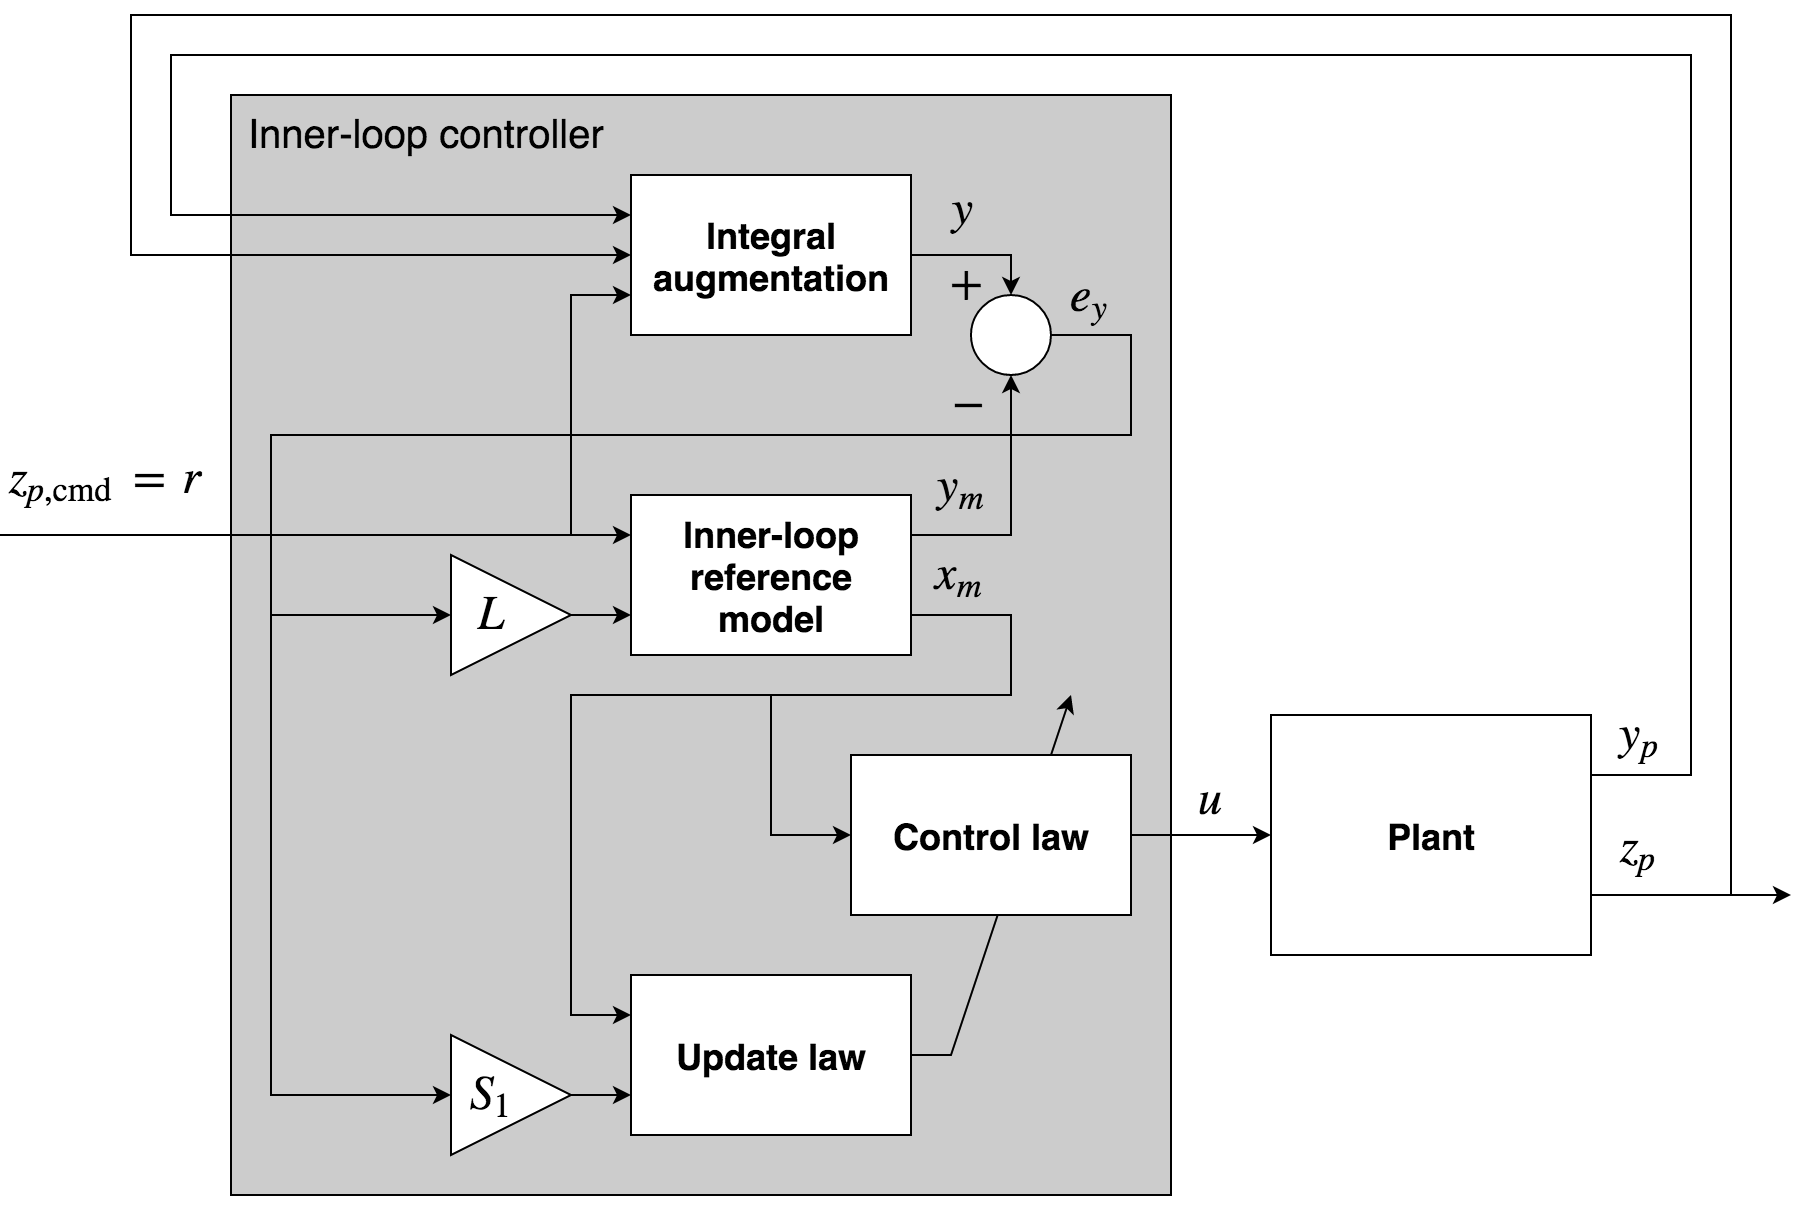
\includegraphics[width=6.5in]{\figurepath/innerLoop2.png}
    \vspace{-0.1in}
    \caption{Inner-loop adaptive control block diagram.\label{fig.innerLoop2}}
  \end{center}
\end{figure}

\begin{rem-dan}
  The calculation of $L$ should conclude with the verification that $A+LC+BK_{x}^{\top}$ is Hurwitz.
  While this is not a theoretical requirement, for practical implementation on systems such as the one presented in the numerical example in Chapter~\ref{ch.applicationHypersonic}, this requirement is enforced to ensure the reference model in\ \eqref{eqn.refmodel} is stable.
\end{rem-dan}

\subsection{Adaptive Law and Stability Proof}\label{sec.adaptivelaw}

Using the closed-loop reference model defined in\ \eqref{eqn.refmodel} with $L$ selected as described in Section~\ref{sec.findingS1andL}, the following update law is proposed:
\begin{equation}
  \label{eqn.updatelaw}
  \dot{\widetilde{\Theta}}(t) = -\Gamma x_{m}(t)\bigr(S_{1}e_{y}(t)\bigr)^{\top}\text{sgn}(\Lambda)
\end{equation}
where $S_{1}$ is chosen using\ \eqref{eqn.S1}.
The closed-loop system is represented using the block diagram shown in Figure~\ref{fig.innerLoop2}.
Alternatively, the inner-loop controller can be represented using the block diagram shown in Figure~\ref{fig.innerLoop3}.

\begin{figure}[H]
  \begin{center}
    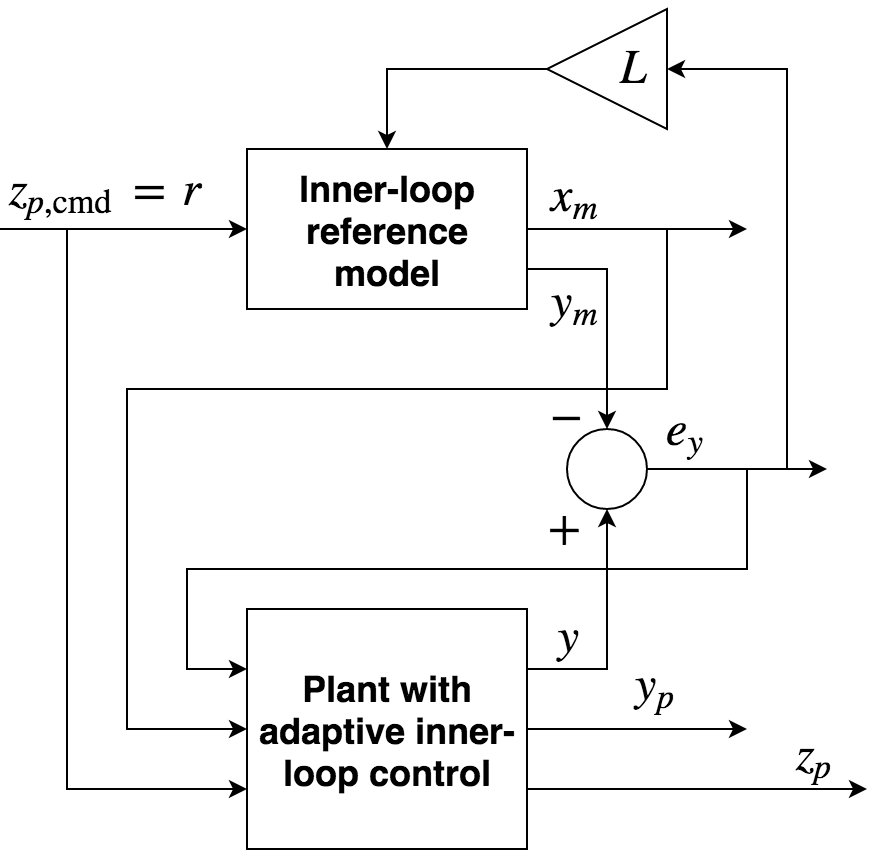
\includegraphics[width=3.5in]{\figurepath/innerLoop3.png}
    \vspace{-0.1in}
    \caption{Inner-loop control block diagram.\label{fig.innerLoop3}}
  \end{center}
\end{figure}

Global stability of the closed-loop system is guaranteed by the following theorem.

\begin{thm-dan}\label{thm.innerLoopStability}
  Given the uncertain linear system in\ \eqref{eqn.uncsystem} which satisfies Assumption~\ref{ass.uncsystem}, the reference model in\ \eqref{eqn.refmodel} with reference input selected as in\ \eqref{eqn.zcmd1}, control law as in\ \eqref{eqn.u}, and the update law in\ \eqref{eqn.updatelaw} results in global stability, with $\lim_{t\rightarrow\infty}e_{x}(t)=0$.
\end{thm-dan}

\begin{proof-dan}
  With a radially unbounded Lyapunov function candidate
  \begin{equation}
    \label{eqn.lyapfunction}
    V\bigr(e_{x}(t),\widetilde{\Theta}(t)\bigr) = e_{x}^{\top}(t)P_{x}e_{x}(t)+\text{tr}\bigr(|\Lambda|\widetilde{\Theta}^{\top}(t)\Gamma^{-1}\widetilde{\Theta}(t)\bigr)
  \end{equation}
  where the operation $|\cdot|$ takes the absolute value of each entry of the matrix argument, a time-derivative $\dot{V}\bigr(e_{x}(t),\widetilde{\Theta}(t)\bigr)$ is obtained as
  \begin{equation*}
    \dot{V}\bigr(e_{x}(t),\widetilde{\Theta}(t)\bigr) = \dot{e}_{x}^{\top}(t)P_{x}e_{x}(t)+e_{x}^{\top}(t)P_{x}\dot{e}_{x}(t)+\text{tr}\bigr(|\Lambda|\dot{\widetilde{\Theta}}^{\top}(t)\Gamma^{-1}\widetilde{\Theta}(t)\bigr)+\text{tr}\bigr(|\Lambda|\widetilde{\Theta}^{\top}(t)\Gamma^{-1}\dot{\widetilde{\Theta}}(t)\bigr)
  \end{equation*}
  Substituting in the error dynamics from\ \eqref{eqn.uncerrdyn} where $A_{L} = A + LC + B\Psi^{\top}$ the Lyapunov candidate derivative $\dot{V}\bigr(e_{x}(t),\widetilde{\Theta}(t)\bigr)$ is written
  \begin{equation*}
    \begin{split}
      \dot{V}\bigr(e_{x}(t),\widetilde{\Theta}(t)\bigr)
      &=
      \bigr(A_{L}e_{x}(t)+B\Lambda\widetilde{\Theta}^{\top}(t)x_{m}(t)\bigr)^{\top}P_{x}e_{x}(t)+e_{x}^{\top}(t)P_{x}\bigr(A_{L}e_{x}(t)+B\Lambda\widetilde{\Theta}^{\top}(t)x_{m}(t)\bigr) \\
      & \qquad + 2\text{tr}\bigr(|\Lambda|\widetilde{\Theta}^{\top}(t)\Gamma^{-1}\dot{\widetilde{\Theta}}(t)\bigr) \\
      %
      &=
      e_{x}^{\top}(t)A_{L}^{\top}P_{x}e_{x}(t) + e_{x}^{\top}(t)P_{x}A_{L}e_{x}(t)+2e_{x}^{\top}(t)PB\Lambda\widetilde{\Theta}^{\top}(t)x_{m}(t) \\
      & \qquad + 2\text{tr}\bigr(|\Lambda|\widetilde{\Theta}^{\top}(t)\Gamma^{-1}\dot{\widetilde{\Theta}}(t)\bigr) \\
      %
      &=
      e_{x}^{\top}(t)(A_{L}^{\top}P_{x}+P_{x}A_{L})e_{x}(t) + 2e_{x}^{\top}(t)P_{x}B\Lambda\widetilde{\Theta}^{\top}(t)x_{m}(t) \\
      & \qquad + 2\text{tr}\bigr(|\Lambda|\widetilde{\Theta}^{\top}(t)\Gamma^{-1}\dot{\widetilde{\Theta}}(t)\bigr) \\
    \end{split}
  \end{equation*}
  Let $A_{L}^{\top}P+PA_{L}=-Q_{x}<0$ as assured by the selection of $L$ satisfying\ \eqref{eqn.lyapal} giving
  \begin{equation*}
    \dot{V}\bigr(e_{x}(t),\widetilde{\Theta}(t)\bigr)
    =
    -e_{x}^{\top}(t)Q_{x}e_{x}(t) + 2e_{x}^{\top}(t)P_{x}B\Lambda\widetilde{\Theta}^{\top}(t)x_{m}(t)+2\text{tr}\bigr(|\Lambda|\widetilde{\Theta}^{\top}(t)\Gamma^{-1}\dot{\widetilde{\Theta}}(t)\bigr)
  \end{equation*}
  Substituting the update law given in\ \eqref{eqn.updatelaw} results in
  \begin{equation*}
    \begin{split}
      \dot{V}\bigr(e_{x}(t),\widetilde{\Theta}(t)\bigr)
      &=
      -e_{x}^{\top}(t)Q_{x}e_{x}(t) + 2e_{x}^{\top}(t)C^{\top}S_{1}^{\top}\Lambda\widetilde{\Theta}^{\top}(t)x_{m}(t) \\
      & \qquad + 2\text{tr}\bigr(|\Lambda|\widetilde{\Theta}^{\top}(t)\Gamma^{-1}\bigr(-\Gamma x_{m}(t)e_{y}^{\top}(t)S_{1}^{\top}\text{sgn}(\Lambda)\bigr)\bigr) \\
      &=
      -e_{x}^{\top}(t)Q_{x}e_{x}(t) + 2e_{s}^{\top}(t)\Lambda\widetilde{\Theta}^{\top}(t)x_{m}(t) - 2\text{tr}\bigr(|\Lambda|\widetilde{\Theta}^{\top}(t)x_{m}(t)e_{y}^{\top}(t)S_{1}^{\top}\text{sgn}(\Lambda)\bigr) \\
      &=
      -e_{x}^{\top}(t)Q_{x}e_{x}(t) + 2e_{s}^{\top}(t)\Lambda\widetilde{\Theta}^{\top}(t)x_{m}(t) - 2\text{tr}\bigr(e_{s}^{\top}(t)\Lambda\widetilde{\Theta}^{\top}(t)x_{m}(t)\bigr) \\
      &=
      -e_{x}^{\top}(t)Q_{x}e_{x}(t) \\
    \end{split}
  \end{equation*}
  Which implies that $V\bigr(e_{x}(t),\widetilde{\Theta}(t)\bigr)$ is a Lyapunov function.
  Since $V\bigr(e_{x}(t),\widetilde{\Theta}(t)\bigr)\succ0$ and $\dot{V}\bigr(e_{x}(t),\widetilde{\Theta}(t)\bigr)\preceq0$, it follows that $V(t)\leq V(0)<\infty$.
  Thus $V(t)\in\mathcal{L}_{\infty}$ which implies $e_{x}(t), \; \widetilde{\Theta}(t)\in\mathcal{L}_{\infty}$.
  Since $z_{p,\text{cmd}}(t),\;e_{x}(t)\in\mathcal{L}_{\infty}$ and the reference model is stable, $x_{m}(t)\in\mathcal{L}_{\infty}$, which implies that $x(t)\in\mathcal{L}_{\infty}$.
  Furthermore,
  \begin{equation*}
    \int_{0}^{t}\dot{V}(\tau)d\tau=V(t)-V(0)
  \end{equation*}
  and since $V\bigr(e_{x}(t),\widetilde{\Theta}(t)\bigr)$ is non increasing and positive definite, $V(0)-V(t)\leq V(0)$.
  This gives
  \begin{equation*}
    -\int_{0}^{t}\dot{V}(\tau)d\tau\leq V(0)
  \end{equation*}
  Substituting in the expression for
  \begin{equation*}
    \dot{V}\bigr(e_{x}(t),\widetilde{\Theta}(t)\bigr) = -e_{x}^{\top}(t)Q_{x}e_{x}(t)
  \end{equation*}
  gives
  \begin{equation*}
    \int_{0}^{t}e_{x}(\tau)^{\top}Q_{x}e_{x}(\tau)d\tau\leq V(0)
  \end{equation*}
  and in turn that $e_{x}(t)\in\mathcal{L}_{2}$.
  Finally, looking at\ \eqref{eqn.uncerrdyn} with $e_{x}(t), \; \widetilde{\Theta}(t), \;\text{and } x_{m}(t)\in\mathcal{L}_{\infty}$ it follows that $\dot{e}_{x}(t)\in\mathcal{L}_{\infty}$.
  With this, it can be concluded using Barbalat's Lemma\ \cite{narendra.stable.2005} that $\lim_{t\rightarrow\infty}e_{x}(t)=0$.
  Since\ \eqref{eqn.lyapfunction} is radially unbounded stability is global.
\end{proof-dan}

\begin{rem-dan}
  The use of the closed-loop reference model in\ \eqref{eqn.refmodel} in no way compromises stability of the closed-loop system.
  Furthermore, with $e_{x}(t)\rightarrow0$ asymptotically as $t\rightarrow\infty$, the term $L\bigr(y_{m}(t)-y(t)\bigr)$ in\ \eqref{eqn.refmodel} tends to zero asymptotically, which in turn indicates that the output of the closed-loop reference model in\ \eqref{eqn.refmodel} tracks that of an open loop reference model, given by\ \eqref{eqn.refmodel} with $L=0$, asymptotically.
  The transient response of the closed-loop reference model as compared with its open-loop counterpart have been discussed in\ \cite{gibson.acc.2013,gibson.ecc.2013,gibson.ieeeaccess.2013}.
  Bounded reference tracking of $z_{p,\text{cmd}}(t)$ by $z_{p}(t)$ follows from  the stability of the closed-loop system as described in the Corollary~\ref{cor.zpcmdtracking} below.
\end{rem-dan}

\begin{cor-dan}\label{cor.zpcmdtracking}
  The inner-loop regulated output $z_{p}(t)$ tracks the inner-loop reference model regulated output $z_{pm}(t)$ asymptotically.
  Furthermore, for piecewise constant commands $z_{p,\text{cmd}}(t)$, the regulated output $z_{p}(t)$ tracks $z_{p,\text{cmd}}(t)$ asymptotically.
\end{cor-dan}

\begin{proof-dan}
  From $\lim_{t\rightarrow\infty}e_{x}(t)=0$ it follows that $\lim_{t\rightarrow\infty}\bigr(x_{e}(t)-x_{em}(t)\bigr) = 0$ where $x_{e}(t)$ is defined in\ \eqref{eqn.xedot} and $x_{em}(t)$ is defined in\ \eqref{eqn.uncertainssRefModel} as $\dot{x}_{em}(t) = z_{p,\text{cmd}}(t) - z_{pm}(t) + L_{e}\bigr(y_{m}(t)-y(t)\bigr)$.
  With this, the following limit can be written
  \begin{equation*}
    \lim_{t\rightarrow\infty}
    \left(
    \int_{0}^{t} \bigr(z_{p,\text{cmd}}(\tau) - z_{p}(\tau)\bigr) d\tau - \int_{0}^{t} \bigr(z_{p,\text{cmd}} - z_{pm}(\tau) + L_{e}C\bigr(x_{m}(\tau)-x(\tau)\bigr)\bigr) d\tau
    \right) = 0
  \end{equation*}
  simplifying
  \begin{equation}
    \label{eqn.intezp}
    \lim_{t\rightarrow\infty}
    \int_{0}^{t} \bigr(z_{p}(\tau) - z_{pm}(\tau)\bigr) d\tau
    =
    \lim_{t\rightarrow\infty}
    L_{e}C \int_{0}^{t} e_{x}(\tau) d\tau < \infty
  \end{equation}
  where the error $e_{zp}(t)$ is given by
  \begin{equation*}
    e_{zp}(t) = z_{p}(t) - z_{pm}(t)
  \end{equation*}
  Recall now that the goal is to show $\lim_{t\rightarrow\infty}e_{zp}(t)=0$.
  Writing out the expression for $e_{zp}(t)$, it follows that
  \begin{equation*}
    e_{zp}(t) = C_{z}x(t) + D_{pz}\bigr(\Lambda u(t) + \Psi^{\top}x(t)\bigr) - C_{z}x_{m}(t) - D_{pz}u_{\text{bl}}(t)
  \end{equation*}
  with $u(t)$ in\ \eqref{eqn.u} and $u_{\text{bl}}(t)$ in\ \eqref{eqn.ubl} the error $e_{zp}(t)$ can be written as
  \begin{equation}
    \label{eqn.ezp}
    \begin{split}
      e_{zp}(t)
      &=
      C_{z}x(t) + D_{pz}\bigr(\Lambda \bigr(K_{x}+\Theta(t)\bigr)^{\top}x_{m}(t)+\Psi^{\top}x(t)\bigr) - C_{z}x_{m}(t) - D_{pz}K_{x}^{\top}x_{m}(t) \\
      &=
      C_{z}e_{x}(t) + D_{pz}\bigr(\Lambda \bigr(K_{x}+\widetilde{\Theta}(t)+\Theta^{*}\bigr)^{\top}x_{m}(t) + \Psi^{\top}x(t) - K_{x}^{\top}x_{m}(t)\bigr) \\
      &=
      C_{z}e_{x}(t) + D_{pz}\bigr(\Lambda \bigr(K_{x}+\Theta^{*}\bigr)^{\top}x_{m}(t) + \Lambda\widetilde{\Theta}^{\top}x_{m}(t)+\Psi^{\top}x(t) - K_{x}^{\top}x_{m}(t)\bigr) \\
    \end{split}
  \end{equation}
  Taking the time derivative of\ \eqref{eqn.ezp} gives
  \begin{equation}
    \label{eqn.ezpdot}
    \dot{e}_{zp}(t)
    =
    C_{z}\dot{e}_{x}(t) + D_{pz}\bigr(\Lambda\bigr(K_{x}+\Theta^{*}\bigr)^{\top}\dot{x}_{m}(t) + \Lambda(\dot{\widetilde{\Theta}}^{\top}(t)x_{m}(t)+\widetilde{\Theta}^{\top}(t)\dot{x}_{m}(t))+\Psi^{\top}\dot{x}(t) - K_{x}^{\top}\dot{x}_{m}(t)\bigr)
  \end{equation}
  Recall Barbalat's Lemma\ \cite{slotine.appliednonlinear.1991}: If a function $f(t)$ has a finite limit as $t\rightarrow\infty$ and if $\dot{f}(t)$ is uniformly continuous (which is equivalent to $\ddot{f}(t)$ being bounded) then $\lim_{t\rightarrow\infty}\dot{f}(t)=0$.
  For this application, let $f(t)=\int_{0}^{t} e_{zp}(\tau) d\tau$ and $\dot{f}(t)=e_{zp}(t)$ and $\ddot{f}(t)=\dot{e}_{zp}(t)$.
  From\ \eqref{eqn.intezp} the function $f(t)$ has a finite limit as $t\rightarrow\infty$.
  Looking at $\ddot{f}(t)=\dot{e}_{z}(t)$ in\ \eqref{eqn.ezpdot}, all of the arguments are bounded, so $\dot{e}_{zp}(t)$ is bounded.
  Thus $\lim_{t\rightarrow\infty}\dot{f}(t)=0$ which is equivalent to $\lim_{t\rightarrow\infty}e_{zp}(t)=0$ as desired.

  Furthermore, with the embedded integrator, the reference model in\ \eqref{eqn.refmodel}, is a type 1 system with respect to the command input.
  With this, the tracking error tending to zero asymptotically as $\lim_{t\rightarrow\infty}e_{x}(t)=0$, and the reference model input in\ \eqref{eqn.zcmd1}, it follows that $z_{pm}(t)\rightarrow z_{p,\text{cmd}}(t)$ as $t\rightarrow\infty$ for piecewise constant commands $z_{p,\text{cmd}}(t)$.
  From this, it follows that $z_{p}(t)\rightarrow z_{p,\text{cmd}}(t)$ asymptotically as $t\rightarrow\infty$, thus satisfying the control goal as desired.
\end{proof-dan}

\begin{rem-dan}
  Corollary~\ref{cor.zpcmdtracking} provides the expected tracking result, in that asymptotic tracking of an arbitrary bounded command $z_{p,\text{cmd}}(t)$ is not possible.
  For example, if the command is a square wave, the best tracking performance that can be achieved is by enforcing the plant to track a suitably filtered version of the command signal.
  In this way, the reference model is essentially serving as a command pre-filter.
\end{rem-dan}

\begin{rem-dan}
  When compared to the existing CRM based adaptive control approaches\ \cite{lavretsky.output.2010, lavretskywise.book.2013, qu.gnc.2013}, the  CRM based method presented in this thesis offers an approach which is computationally simpler, requiring primarily finding nullspaces of some matrices, as described in the step-by-step procedure in Section~\ref{sec.designprocedure}.
\end{rem-dan}

In the following section the applicability of the CRM based method as compared to the classical MIMO adaptive control method is examined.

\section{Comparison Between CRM Based and Classical MIMO Adaptive Control}\label{sec.AdaptiveComparison}

Given the classical approaches used in the  literature thus far, the obvious question that is raised is how the proposed MIMO controller fares compared to the classical ones.
The first point to note here is that the classical approaches are limited to square plants while the approach proposed here is not.
This is the most obvious advantage of this method.
The next question that arises is a comparison of the two approaches when the underlying plant is square.
This is addressed below.

As a first step, the relevant definitions are provided below:

\begin{defn-dan}[(Markov Parameters)]\cite{antsaklis.linearsystems.2006}\label{defn.markov}
  Given a transfer matrix $G(s)$, the \textit{Markov Parameters} are given by
  \begin{equation*}
    H_{0}=\lim_{s\rightarrow\infty}G(s),
    \qquad
    H_{1}=\lim_{s\rightarrow\infty}s(G(s)-H_{0}),
    \qquad
    H_{2}=\lim_{s\rightarrow\infty}s^{2}(G(s)-H_{0}-H_{1}s^{-1})
  \end{equation*}
  and so forth.
\end{defn-dan}

\begin{thm-dan}\label{thm.markov_realization}
  The set $(A,B,C,D)$ is a realization of $G(s)$ if and only if
  \begin{equation*}
    H_{0}=D
    \qquad
    H_{i}=CA^{i-1}B, \quad i=1,2,\dots
  \end{equation*}
\end{thm-dan}

\begin{proof-dan}
  The proof can be found in Reference\ \cite{antsaklis.linearsystems.2006}.
\end{proof-dan}

\begin{defn-dan}
  \textbf{(Relative Degree One)}\label{defn.relativedegreeone}
  The MIMO system $G(s)$ with realization $(A,B,C,D)$ is said to be Relative Degree One if $H_{0}=0$ and $H_{1}=CB$ is full rank.
\end{defn-dan}

\begin{lem-dan}\label{lem.E}
  Reference\ \cite{narendra.stable.2005}
  Given a square nonsingular strictly proper transfer matrix $W_{p}(s)\in\mathbb{R}_{p}^{m\times m}(s)$, its Hermite form is diagonal if and only if the constant matrix $E(W_{p}(s))$ is nonsingular, where $E$ is calculated as follows.
  Calculate $r_{i}$ as the minimum relative degree in the $i^{\text{th}}$ row of $W_{p}(s)$ and the rows of $E$ are
  \begin{equation}
    \label{eqn.Ei}
    E_{i}=\lim_{s\rightarrow\infty}s^{r_{i}}W_{p,i}(s)
  \end{equation}
  where $W_{p,i}(s)$ corresponds to the $i^{\text{th}}$ row of $W_{p}(s)$.
\end{lem-dan}

\begin{proof-dan}
  The proof can be found in Reference\ \cite{chen.introduction.1970}
\end{proof-dan}

Given $W_{p}(s)\in\mathbb{R}_{p}^{m\times m}(s)$, the assumptions that must be satisfied for a classical adaptive control solution to exist are as follows\ \cite{narendra.stable.2005}.

\begin{customthm}{2} $\;$\label{ass.classical}
  \begin{enumerate}[(\roman{enumi}), ref=\roman{enumi}]
    \itemsep0em
    \item{The high frequency gain matrix $K_{p}$ is of the form $K_{p}=\overline{K}_{p}\Lambda$ where $\overline{K}_{p}$ is known and $\text{sign}(\Lambda)$ is known.\label{ass.kp}}
    \item{The right Hermite normal form $H_{p}(s)$ of $W_{p}(s)$ is known.\label{ass.hermite}}
    \item{An upper bound $\nu$ on the observability index of $W_{p}(s)$ is known.\label{ass.nu}}
    \item{The zeros of $W_{p}(s)$ lie in $\mathbb{C}^{-}$.\label{ass.tzeroWp}}
  \end{enumerate}
\end{customthm}

\begin{thm-dan}\label{thm.CB}
  Given the square plant $W_{p}(s)\in\mathbb{R}_{p}^{m\times m}$ with realization $(A,B,C,0)$, the Hermite form $H_{p}(s)$ of $W_{p}(s)$ is diagonal if $CB$ is full rank.
  Furthermore, the high frequency gain matrix is given by $K_{p}=CB$.
\end{thm-dan}

\begin{proof-dan}
  Theorem~\ref{thm.markov_realization} connects the Markov Parameters of Relative Degree One systems to the realization of $W_{p}(s)$ with $H_{0}=0$ and $H_{1}=CB$.
  With this and Definition~\ref{defn.markov}, $\lim_{s\rightarrow\infty}sW_{p}(s)=CB$ is full rank, and so the minimum relative degree in each row of $W_{p}(s)$ is $r_{i}=1$.
  By Lemma~\ref{lem.E} $E(W_{p}(s))=CB$ and the Hermite form $H_{p}(s)$ of $W_{p}(s)$ is diagonal.
  In Reference\ \cite{narendra.stable.2005} it is shown that $E(W_{p}(s))=K_{p}$.
\end{proof-dan}

Using Definitions~\ref{defn.markov} and~\ref{defn.relativedegreeone} as well as Theorems~\ref{thm.markov_realization} and~\ref{thm.CB}, it is shown in Proposition~\ref{prop.mimoequiv} that the classical and the CRM based MIMO adaptive control solution in this paper are equally applicable when the system in\ \eqref{eqn.xdotpunc} is square.

\begin{prop-dan}\label{prop.mimoequiv}
  Consider the uncertain system in\ \eqref{eqn.xdotpunc} where $\ell=m$ and the plant transfer matrix is given by
  \begin{equation}
    \label{eqn.wpofs}
    W_{p}(s)=C_{p}(sI-A_{p}-B_{p} \Psi_{p}^{\top})^{-1}B_{p}\Lambda
  \end{equation}
  if the plant in\ \eqref{eqn.xdotpunc} satisfies Assumption~\ref{ass.plant}, then the corresponding $W_p(s)$ in\ \eqref{eqn.wpofs} satisfies Assumption~\ref{ass.classical}.
\end{prop-dan}

\begin{proof-dan}
  Assumption~\ref{ass.plant}\ref{ass.p.unc}-(\ref{ass.p.unc.lambda}) and Theorem~\ref{thm.CB} can be shown to imply that the corresponding $K_p$ satisfies Assumption~\ref{ass.classical}(\ref{ass.kp}).
  Assumption~\ref{ass.plant}\ref{ass.p.rank} together with Theorem~\ref{thm.CB} implies that the corresponding Hermite form is diagonal with known entries and is therefore known, which leads to Assumption~\ref{ass.classical}(\ref{ass.hermite}).
  Assumption~\ref{ass.classical}(\ref{ass.nu}) follows from the fact that $n_{p}$ is known.
  Finally Assumption~\ref{ass.plant}\ref{ass.p.tzero} is equivalent to Assumption~\ref{ass.classical}(\ref{ass.tzeroWp}).
\end{proof-dan}

In addition to the main advantage of the proposed method of applicability to non-square plants, the proposed controller is of lower order, requiring only $n$ controller states and $nm$ adjustable parameters, as compared with the classical solution which will introduce $2m\nu$ states and $2m^{2}\nu$ parameters.
This reduces the number of states and parameters necessary by at least two, since $n\leq\nu m$\ \cite{chen.linear.1999}.
Finally the proposed solution is based on a CRM, which has been shown to possess a superior transient performance\ \cite{gibson.aiaacrm.2012,gibson.acc.2013,gibson.ecc.2013,gibson.ieeeaccess.2013}.

It should be noted that of Assumptions~\ref{ass.plant}\ref{ass.p.cont}-\ref{ass.p.unc}, which are required to be satisfied for the proposed controller, the most restrictive one is Assumption~\ref{ass.plant}\ref{ass.p.rank}, which implies that the MIMO system must have Relative Degree One.
In most aerial platforms including hypersonic vehicles, this assumption is easy to satisfy as the relative degree of the transfer functions between the control surface deflections and aircraft angular rates is unity.
Additionally, the structure of the plant as in\ \eqref{eqn.xdotpunc} which has matched uncertainties is also commonly present in flight control applications where much of the plant uncertainty is in the aerodynamic moment coefficients and loss of control effectiveness, which are spanned by the columns of $B$.
It is however required that the uncertainty $\Psi_{p}$ satisfy Assumption~\ref{ass.plant}\ref{ass.p.unc}-(\ref{ass.p.unc.wp}), which is not required in the classical approach.
Note finally that the above comparison between the proposed controller and the classical ones was done for Relative Degree One plants only.
Clearly the classical methods such as those in Reference\ \cite{narendra.stable.2005} are applicable to plants with with larger relative degrees, where the proposed method is not.

\section{Numerical Examples}\label{sec.innerLoopNumericalExample}

\subsection{Example 1: Inverted Pendulum Cart}

Consider the inverted cart-pendulum system as given in Ref.\ \cite{astrom.feedbackintro.2010} and shown in Fig.~\ref{fig.pendulumCart}.

\begin{figure}[H]
  \begin{center}
    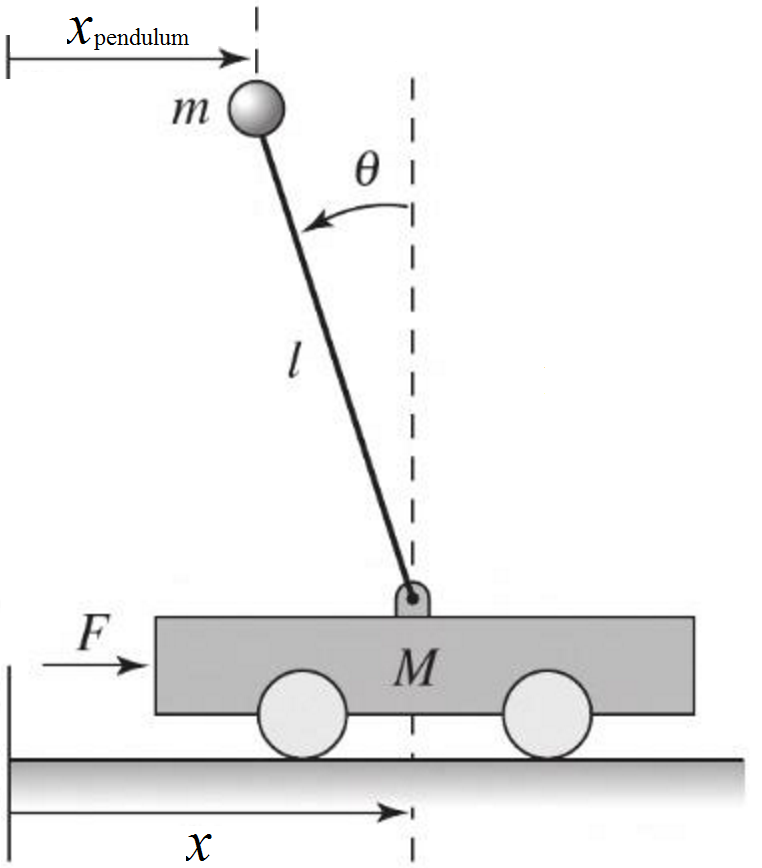
\includegraphics[width=2.8in]{\figurepath/pendulumCart.png}
    \vspace{-0.1in}
    \caption{Inverted pendulum on cart from Ref.\ \cite{astrom.feedbackintro.2010}.\label{fig.pendulumCart}}
  \end{center}
\end{figure}

The linearized equations of motion are given by the following, where $M$ is the mass of the cart, $m$ is the mass of the pendulum, $J$ is the moment of inertia of the pendulum, $l$ is the pendulum length, $c$ and $\gamma$ are coefficients of viscous friction, and $g$ is the acceleration due to gravity.
\begin{equation}
  \label{eqn.pendulumCartWhole}
  \begin{bmatrix}
    \ddot{\theta} \\
    \ddot{x} \\
    \dot{\theta} \\
    \dot{x}
  \end{bmatrix}
  =
  \begin{bmatrix}
    -\frac{\gamma M_{t}}{\mu} & -\frac{cl m}{\mu} & \frac{M_{t}mgl}{\mu} & 0 \\
    -\frac{\gamma J_{t}l m}{\mu} & -\frac{cJ_{t}}{\mu} & \frac{m^{2}g^{2}l}{\mu} & 0 \\
    1 & 0 & 0 & 0 \\
    0 & 1 & 0 & 0 \\
  \end{bmatrix}
  \begin{bmatrix}
    \dot{\theta} \\
    \dot{x} \\
    \theta \\
    x
  \end{bmatrix}
  +
  \begin{bmatrix}
    \frac{l m}{\mu} \\
    \frac{J_{t}}{\mu} \\
    0 \\
    0
  \end{bmatrix}
  F
\end{equation}
where the total mass $M_{t}$ and total moment of inertia $J_{t}$ are given by
\begin{equation*}
  \begin{aligned}
    M_{t} & = M + m \\
    J_{t} &= J + ml^{2}
  \end{aligned}
\end{equation*}
and where $\mu$ is given by
\begin{equation*}
  \mu = M_{t}J_{t} - m^{2}l^{2}
\end{equation*}
Considering uncertainty in the coefficients of viscous friction, this system is represented by Eq.\ \eqref{eqn.wholeSystemUncertain}.
Partitioning\ \eqref{eqn.pendulumCartWhole} as described in Chapter~\ref{ch.Introduction}, the inner-loop dynamics in the form of\ \eqref{eqn.innerLoopDynamicsUncertain} and outer-loop dynamics as in\ \eqref{eqn.outerLoopDynamics} are obtained.
The following numerical values were selected
\begin{equation}
  \label{eqn.pendulumNumericalValues}
  \begin{aligned}
    m &= 1 \text{~kg} \\
    M &= 1 \text{~kg} \\
    l &= 1 \text{~m} \\
    \gamma &= 1 \text{~Ns/m} \\
    c &= 1 \text{~Ns/m} \\
    g &= 9.8 \text{~m/s}^2
  \end{aligned}
\end{equation}
The inner-loop control goal is to stabilize the system using a single velocity measurement.
The velocity of the cart $\dot{x}$ is selected, with this output serving as both the measured and regulated outputs, leading to the following inner-loop dynamics
\begin{equation}
  \label{eqn.pendulumCartInnerLoop}
  \begin{split}
    \begin{bmatrix}
      \ddot{\theta} \\
      \ddot{x}
    \end{bmatrix}
    &=
    \begin{bmatrix}
      -\frac{\gamma M_{t}}{\mu} & -\frac{cl m}{\mu} \\
      -\frac{\gamma J_{t}l m}{\mu} & -\frac{cJ_{t}}{\mu}
    \end{bmatrix}
    \begin{bmatrix}
      \dot{\theta} \\
      \dot{x}
    \end{bmatrix}
    +
    \begin{bmatrix}
      \frac{l m}{\mu} \\
      \frac{J_{t}}{\mu}
    \end{bmatrix}
    F \\
    \dot{x}
    &=
    \begin{bmatrix}
      0 & 1
    \end{bmatrix}
    \begin{bmatrix}
      \dot{\theta} \\
      \dot{x}
    \end{bmatrix}
  \end{split}
\end{equation}
Using the numerical values in\ \eqref{eqn.pendulumNumericalValues}, the system in\ \eqref{eqn.pendulumCartInnerLoop} is given by
\begin{equation*}
  \begin{split}
    \begin{bmatrix}
      \ddot{\theta} \\
      \ddot{x}
    \end{bmatrix}
    &=
    \begin{bmatrix}
      -2 & -1 \\
      -1 & -1
    \end{bmatrix}
    \begin{bmatrix}
      \dot{\theta} \\
      \dot{x}
    \end{bmatrix}
    +
    \begin{bmatrix}
      1 \\
      1
    \end{bmatrix}
    F \\
    \dot{x}
    &=
    \begin{bmatrix}
      0 & 1
    \end{bmatrix}
    \begin{bmatrix}
      \dot{\theta} \\
      \dot{x}
    \end{bmatrix}
  \end{split}
\end{equation*}
The following uncertainty was selected, which is equivalent to the damping coefficient $c=0$, thus making the uncertain system marginally stable, as well as having a reduction in the input to 65\% the nominal control force applied to the cart.
\begin{equation*}
  \begin{split}
    \Psi_{p}
    &=
    \begin{bmatrix}
      0 & 1
    \end{bmatrix}^{\top} \\
    \Lambda
    &=
    0.65
  \end{split}
\end{equation*}
The following weighting matrices were used to design the LQR inner-loop baseline controller
\begin{equation*}
  \begin{split}
    Q_{\text{lqr}}
    &=
    \text{diag}\bigr(
    \begin{bmatrix}
    0 & 0 & 1
    \end{bmatrix}\bigr) \\
    R_{\text{lqr}}
    &=
    10{-6}
  \end{split}
\end{equation*}
The following upper-bound on the uncertainty was used
\begin{equation*}
  \Psi_{\text{max}} = 10
\end{equation*}
resulting in $X$ in\ \eqref{eqn.Px} given by
\begin{equation*}
  X =
  \begin{bmatrix}
    1.1 & 1 \\
    1 & 10
  \end{bmatrix}
\end{equation*}
This inner-loop adaptive controller was then implemented in a simulation of the pendulum model, resulting in the response shown in Fig.~\ref{fig.innerLoopPendulumCart}.
In the following simulations, the simulation begins with the baseline controller applied to the nominal system.
At $t=10$ seconds uncertainty is introduced, while still using only the baseline controller.
At $t=30$ seconds adaptive controller is turned on.
In these simulations, it is important to first note that the oscillations observed in the baseline response are due to the coupling of the kinematics, in this case the pendulum angle, into the dynamics.
While it is often assumed, as described above, that the term associated with this coupling, $B_{gd}$, is negligible, it will still have an impact on the closed-loop performance, except in cases when it is identically zero.
While the nominal response does contain oscillations, they are damped, and steady-state tracking of the piecewise constant cart velocity command is achieved.
When uncertainty is introduced, the oscillations become much larger, and begin to diverge, indicating the uncertainty has made the closed-loop system very lightly damped, and slightly unstable.
The adaptive controller, when turned on, quickly recovers the nominal performance.

\newpage
\begin{figure}[H]
  \hspace{-0.25in}
  \noindent\makebox[7.0in]{%
  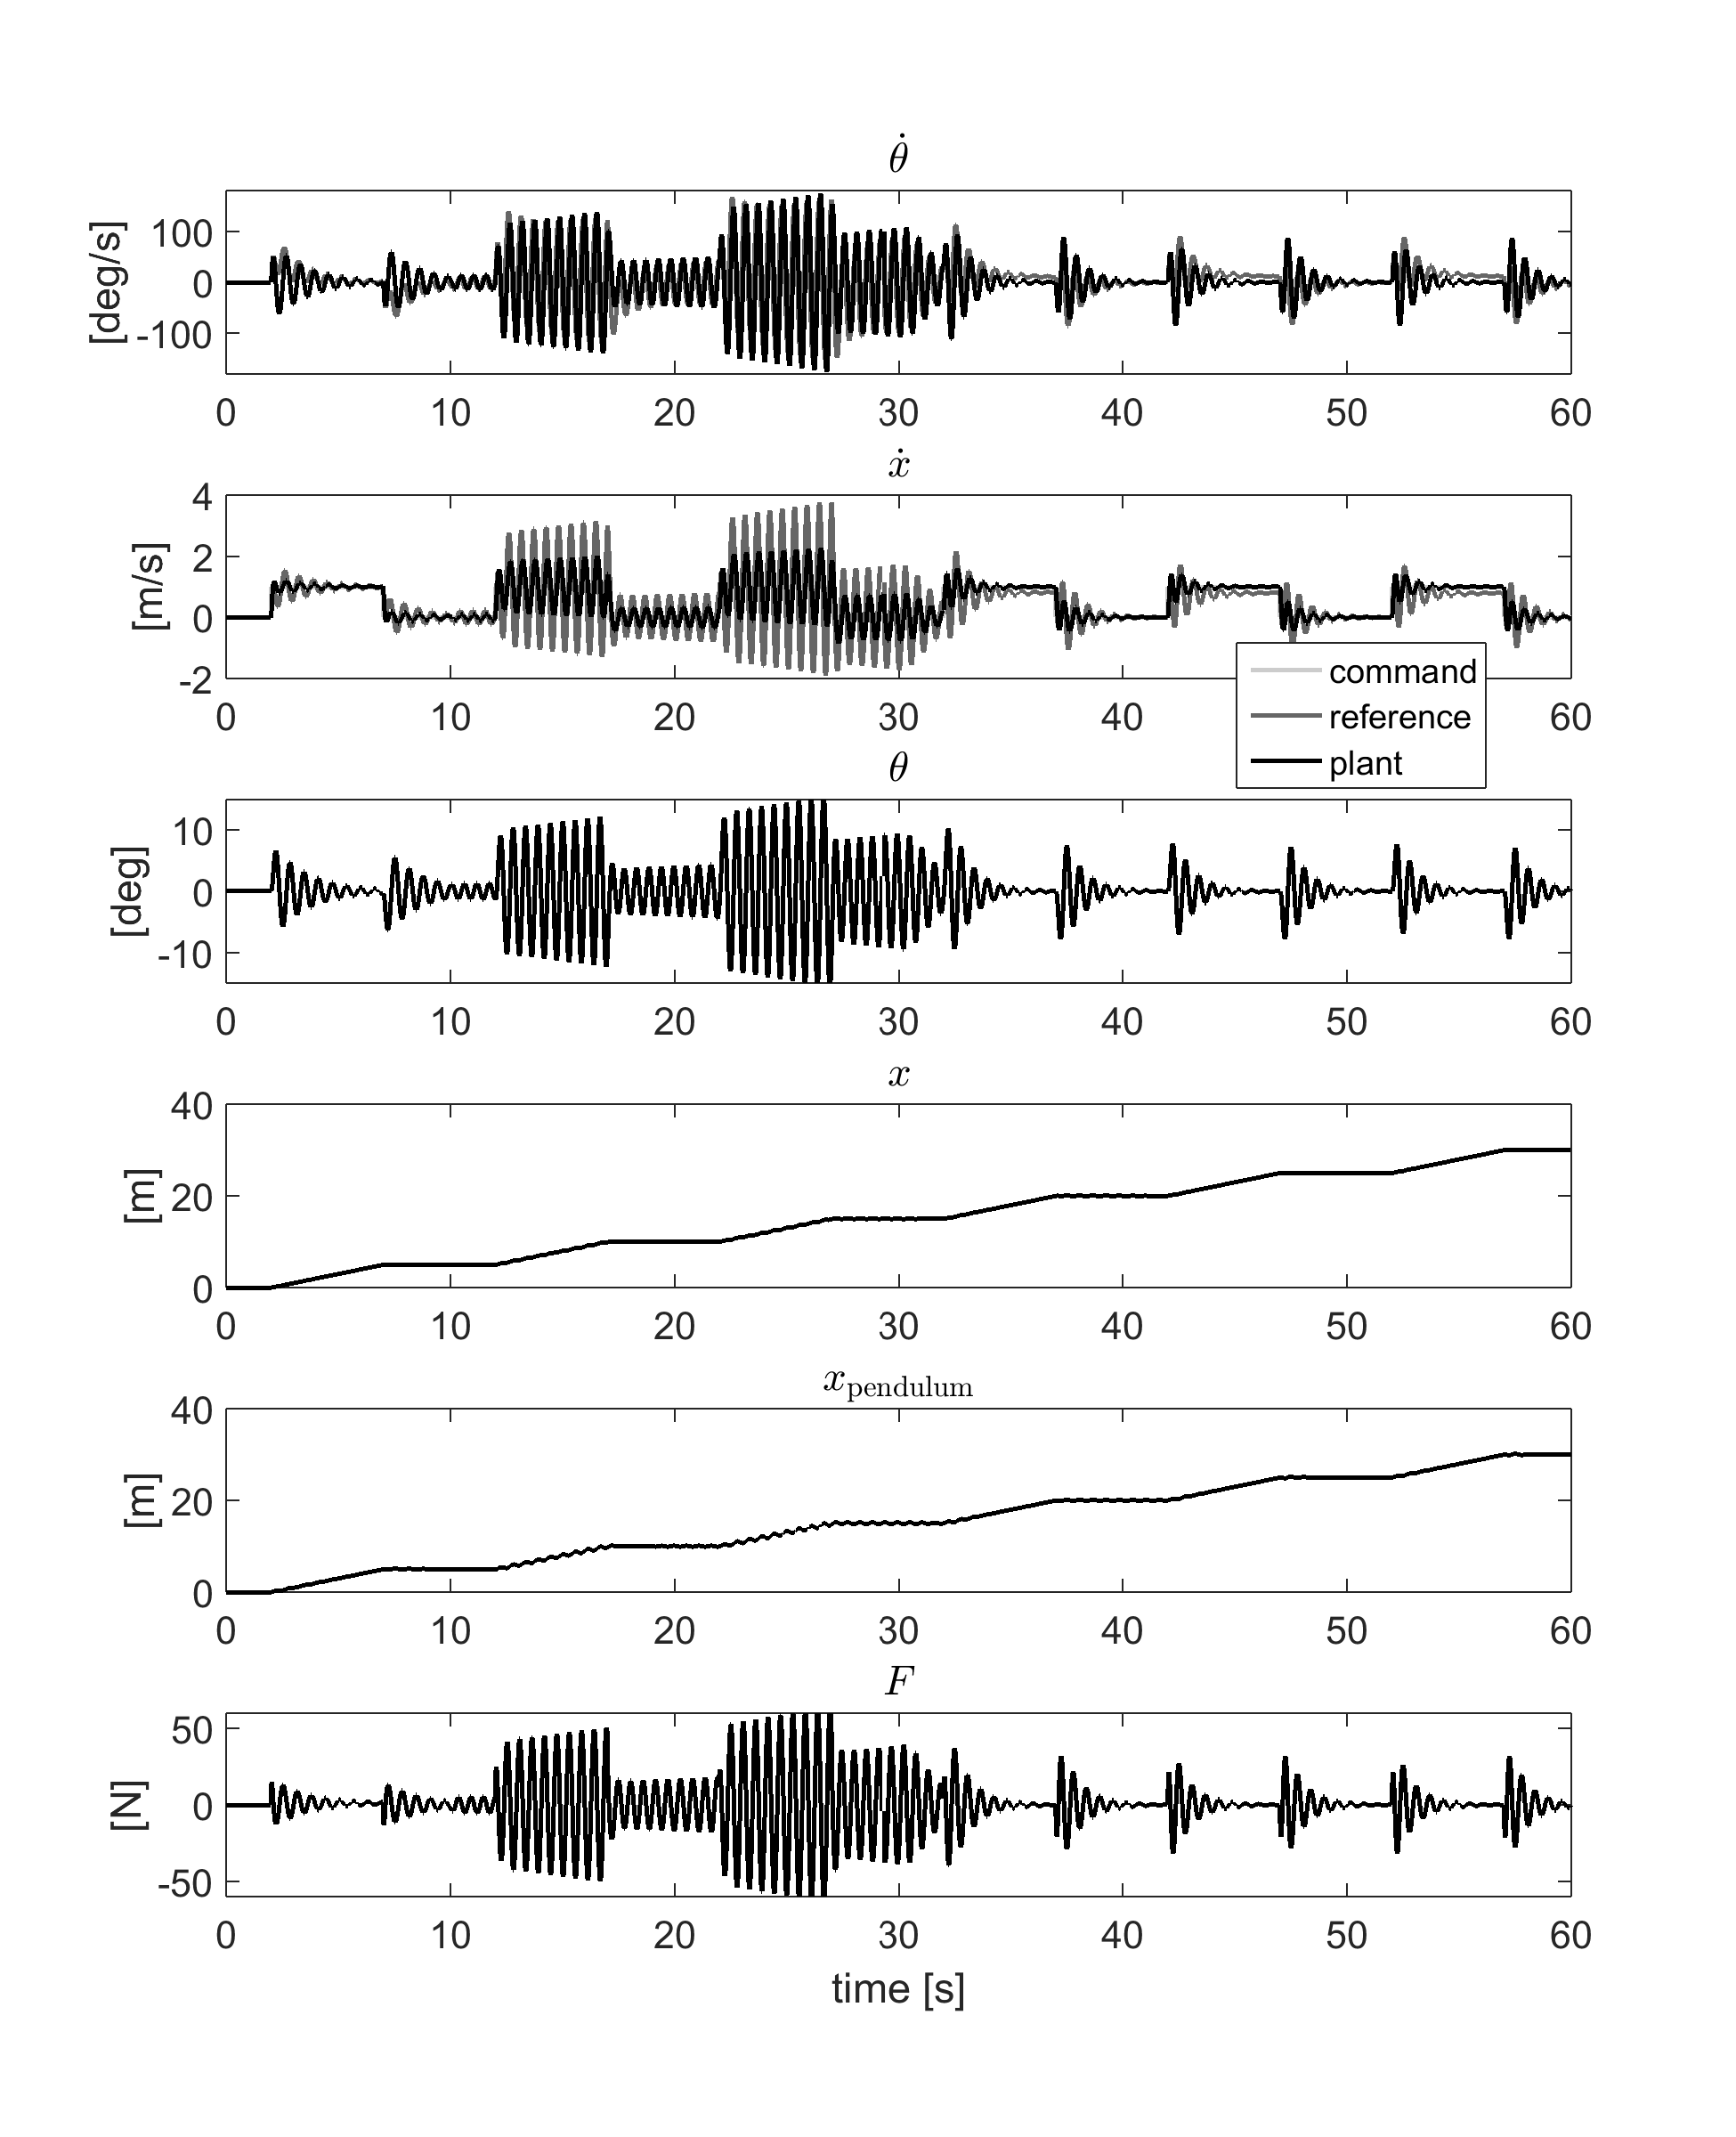
\includegraphics[width=7.0in]{\figurepath/innerLoopPendulumCart.png}}
  \vspace{-0.95in}
  \caption{Time response of pendulum cart with inner-loop controller.\label{fig.innerLoopPendulumCart}}
\end{figure}

\subsection{Example 2: Longitudinal Dynamics of a Transport Aircraft}

For this example, consider the longitudinal dynamics of a transport aircraft, in this case a 747--100.
\begin{figure}[H]
  \begin{center}
    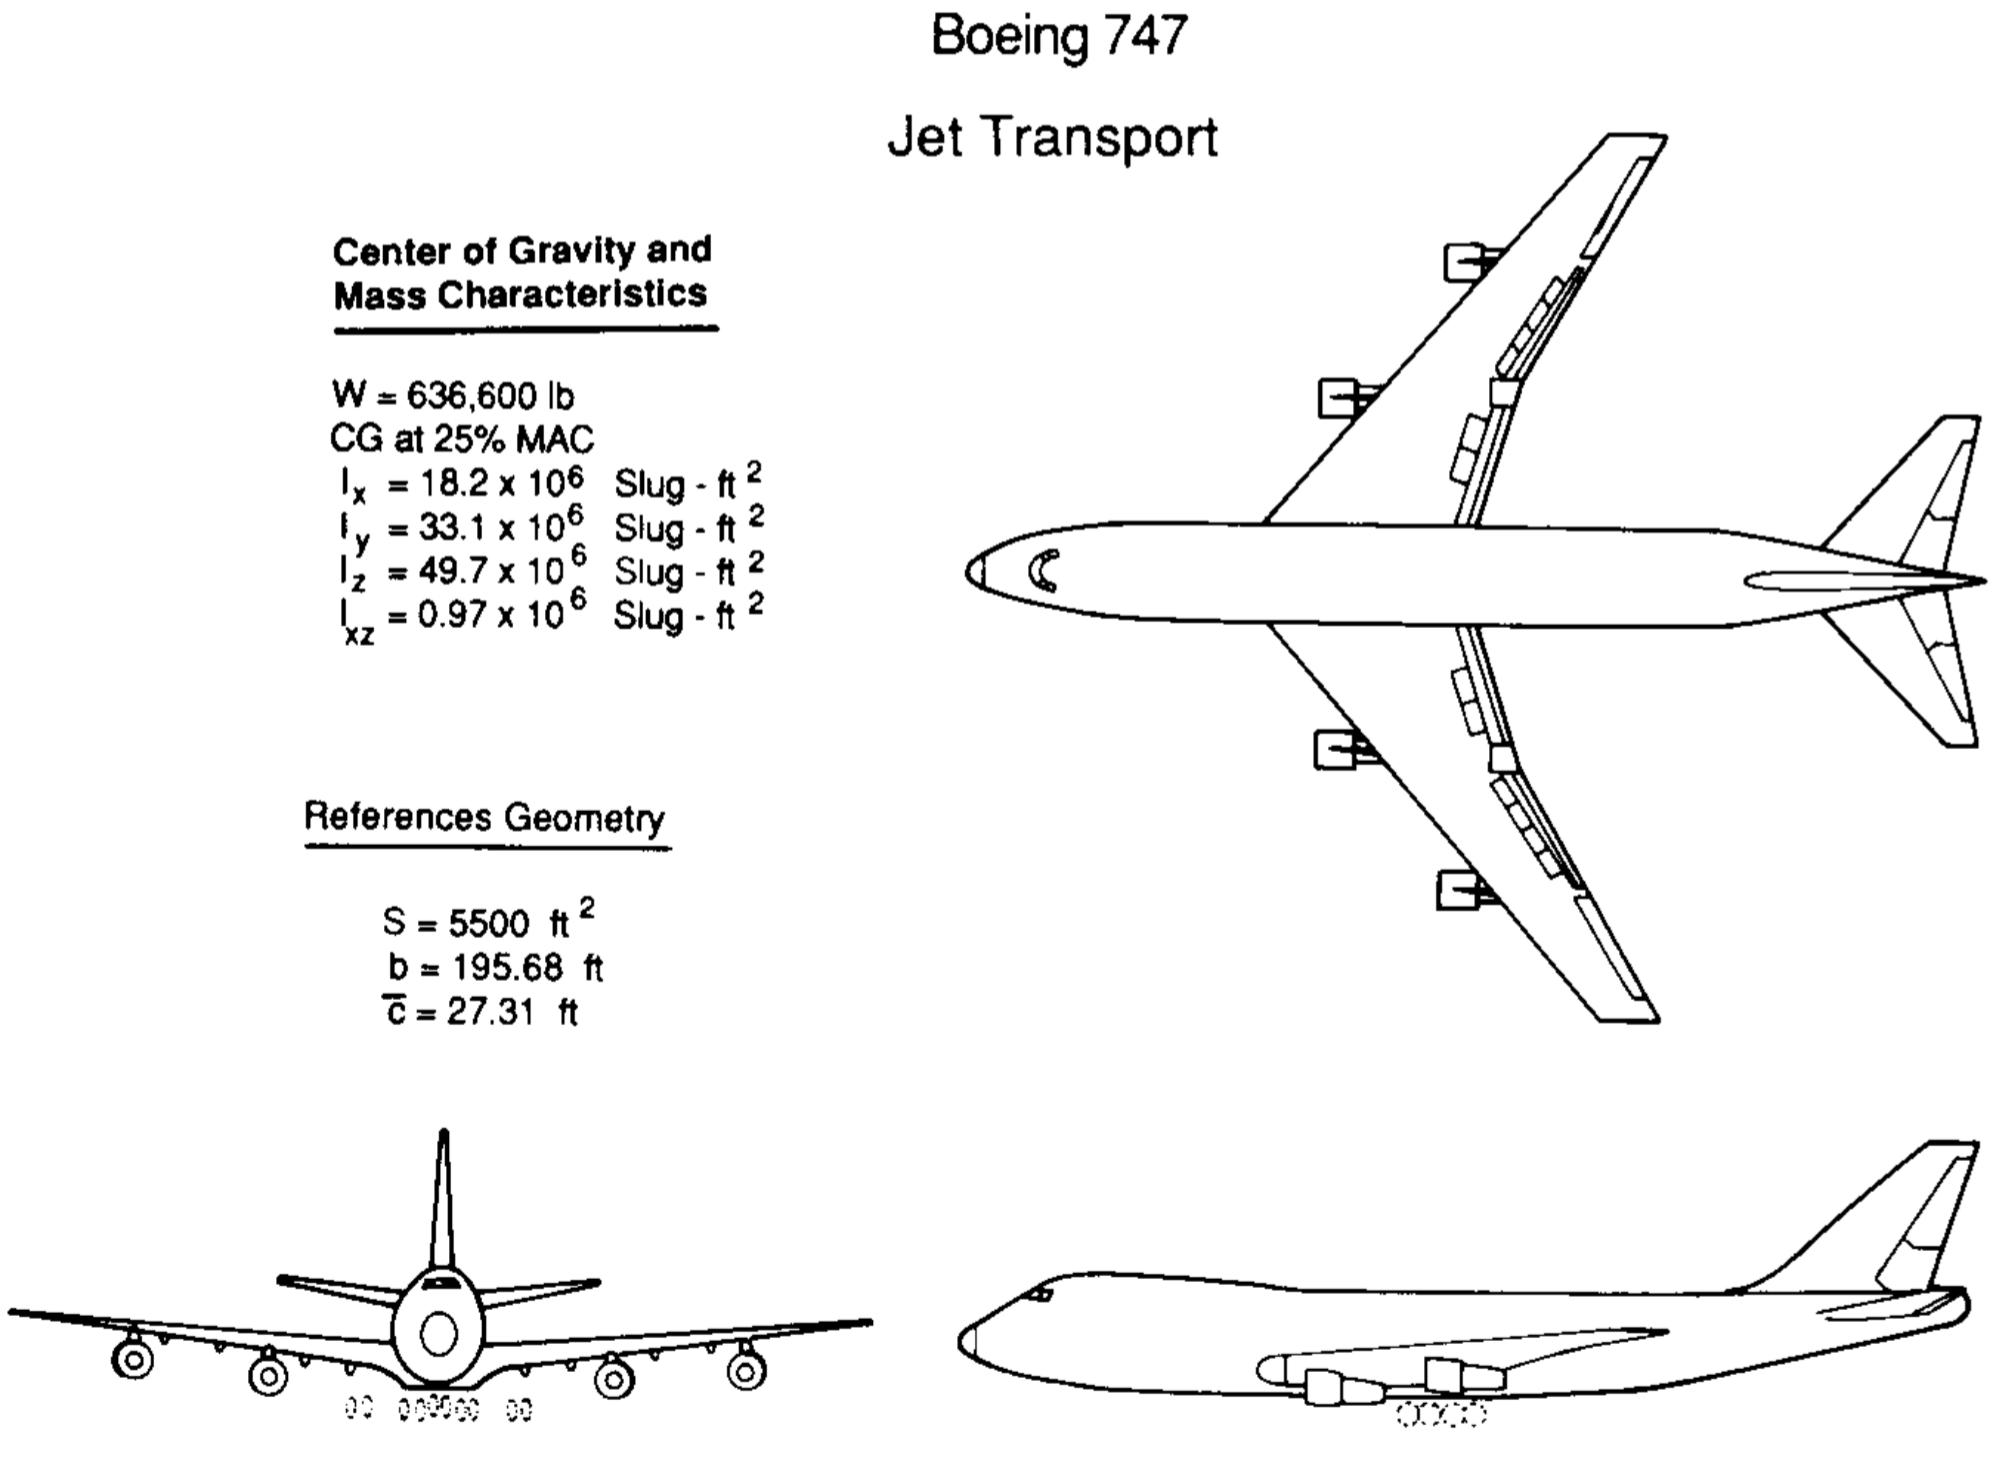
\includegraphics[width=4.5in]{\figurepath/transportLong.png}
    \vspace{-0.1in}
    \caption{Boeing 747--100 transport aircraft from Ref.\ \cite{nelson.flightcontrol.1998}.\label{fig.transportLong}}
  \end{center}
\end{figure}
The equations of motion describing the longitudinal dynamics of a transport aircraft such as the 747--100 during steady, level flight are given by the following
\begin{equation}
  \label{eqn.transportAircraftWhole}
  \begin{bmatrix}
    \dot{\alpha} \\
    \dot{q} \\
    \dot{\theta} \\
    \dot{h}
  \end{bmatrix}=
  \begin{bmatrix}
    \frac{Z_{\alpha}}{v_{\text{eq}}} & 1 & 0 & 0 \\
    M_{\alpha}+\frac{M_{\dot{\alpha}}Z_{\alpha}}{v_{\text{eq}}} & M_{q}+M_{\dot{\alpha}} & 0 & 0 \\
    0 & 1 & 0 & 0 \\
    -v_{\text{eq}} & 0 & v_{\text{eq}} & 0 \\
  \end{bmatrix}
  \begin{bmatrix}
    \alpha \\
    q \\
    \theta \\
    h
  \end{bmatrix}+
  \begin{bmatrix}
    \frac{Z_{\delta_{e}}}{v_{\text{eq}}} \\
    M_{\delta_{e}} \\
    0 \\
    0
  \end{bmatrix}
  \delta_{e}
\end{equation}
where $\alpha$ is the angle-of-attack, $q$ is the pitch rate, $\theta$ the pitch angle, $h$ is the altitude, and $\delta_{e}$ is the elevator deflection angle.
Considering uncertainty in the aerodynamic moment coefficients $M_{\alpha}$ and $M_{q}$, this system is represented by Eq.\ \eqref{eqn.wholeSystemUncertain}.
Partitioning\ \eqref{eqn.transportAircraftWhole} as described in Chapter~\ref{ch.Introduction}, the inner-loop dynamics in the form of\ \eqref{eqn.innerLoopDynamicsUncertain} and outer-loop dynamics as in\ \eqref{eqn.outerLoopDynamics} are obtained.
The following numerical values were selected from Ref.\ \cite{heffley.nasacr2144.1972, nelson.flightcontrol.1998}
\begin{equation*}
  \begin{aligned}
    v_{\text{eq}} &= 871 \text{~ft/s} \\
    Z_{\alpha} &= -349 \text{~ft/s}^{2} \\
    M_{\alpha} &= -1.65 \text{~rad/s}^{2} \\
    M_{\dot{\alpha}} &= -0.139 \text{~rad/s} \\
    M_{q} &= -0.401 \text{~rad/s} \\
    M_{\delta_{e}} &= -1.22 \text{~rad/s}^{2} \\
    Z_{\delta_{e}} &= -18.6 \text{~ft/s}^{2}
  \end{aligned}
\end{equation*}
The inner-loop control goal is to stabilize the system using only pitch rate measurement, with this output serving as both the measured and regulated outputs, leading to the following inner-loop dynamics
\begin{equation}
  \label{eqn.transportAircraftInnerLoop}
  \begin{split}
    \begin{bmatrix}
      \dot{\alpha} \\
      \dot{q}
    \end{bmatrix}
    &=
    \begin{bmatrix}
      \frac{Z_{\alpha}}{v_{\text{eq}}} & 1 \\
      M_{\alpha}+\frac{M_{\dot{\alpha}}Z_{\alpha}}{v_{\text{eq}}} & M_{q}+M_{\dot{\alpha}} \\
    \end{bmatrix}
    \begin{bmatrix}
    \alpha \\
    q
    \end{bmatrix}+
    \begin{bmatrix}
      \frac{Z_{\delta_{e}}}{v_{\text{eq}}} \\
      M_{\delta_{e}}
    \end{bmatrix}
    \delta_{e} \\
    q &=
    \begin{bmatrix}
      0 & 1
    \end{bmatrix}
    \begin{bmatrix}
    \alpha \\
    q
    \end{bmatrix}
  \end{split}
\end{equation}
The following uncertainty was selected, which is equivalent to uncertainty in the moment coefficients.
In addition, there is a reduction in the control effectiveness of the elevator to 50\% its nominal value.
\begin{equation*}
  \begin{split}
    \Psi_{p}
    &=
    \begin{bmatrix}
      4 & -4
    \end{bmatrix}^{\top} \\
    \Lambda
    &=
    0.5
  \end{split}
\end{equation*}
The following weighting matrices were used to design the LQR inner-loop baseline controller
\begin{equation*}
  \begin{split}
    Q_{\text{lqr}}
    &=
    \text{diag}\bigr(
    \begin{bmatrix}
      0 & 0 & 1000
    \end{bmatrix}\bigr) \\
    R_{\text{lqr}}
    &=
    1
  \end{split}
\end{equation*}
The following upper-bound on the uncertainty was used
\begin{equation*}
  \Psi_{\text{max}} = 1000
\end{equation*}
resulting in $X$ in\ \eqref{eqn.Px} given by
\begin{equation*}
  X =
  \begin{bmatrix}
    1.0005 & 1 \\
    1 & 2199
  \end{bmatrix}
\end{equation*}
This inner-loop adaptive controller was then implemented in a simulation of the aircraft model, resulting in the response shown in Fig.~\ref{fig.innerLoopTransportLong}.
Unlike the pendulum model, the kinematics of the aircraft, the pitch angle and altitude, do not couple into the inner-loop short-period dynamics at all.
Thus, the assumption that $B_{gd}=0$ in Eq.\ \eqref{eqn.wholeSystemUncertain} is satisfied exactly.
At $t=10$ seconds uncertainty is introduced, but the adaptive controller is not activated until $t=30$ seconds.

\newpage
\begin{figure}[H]
  \hspace{-0.0in}
  \noindent\makebox[6.5in]{%
  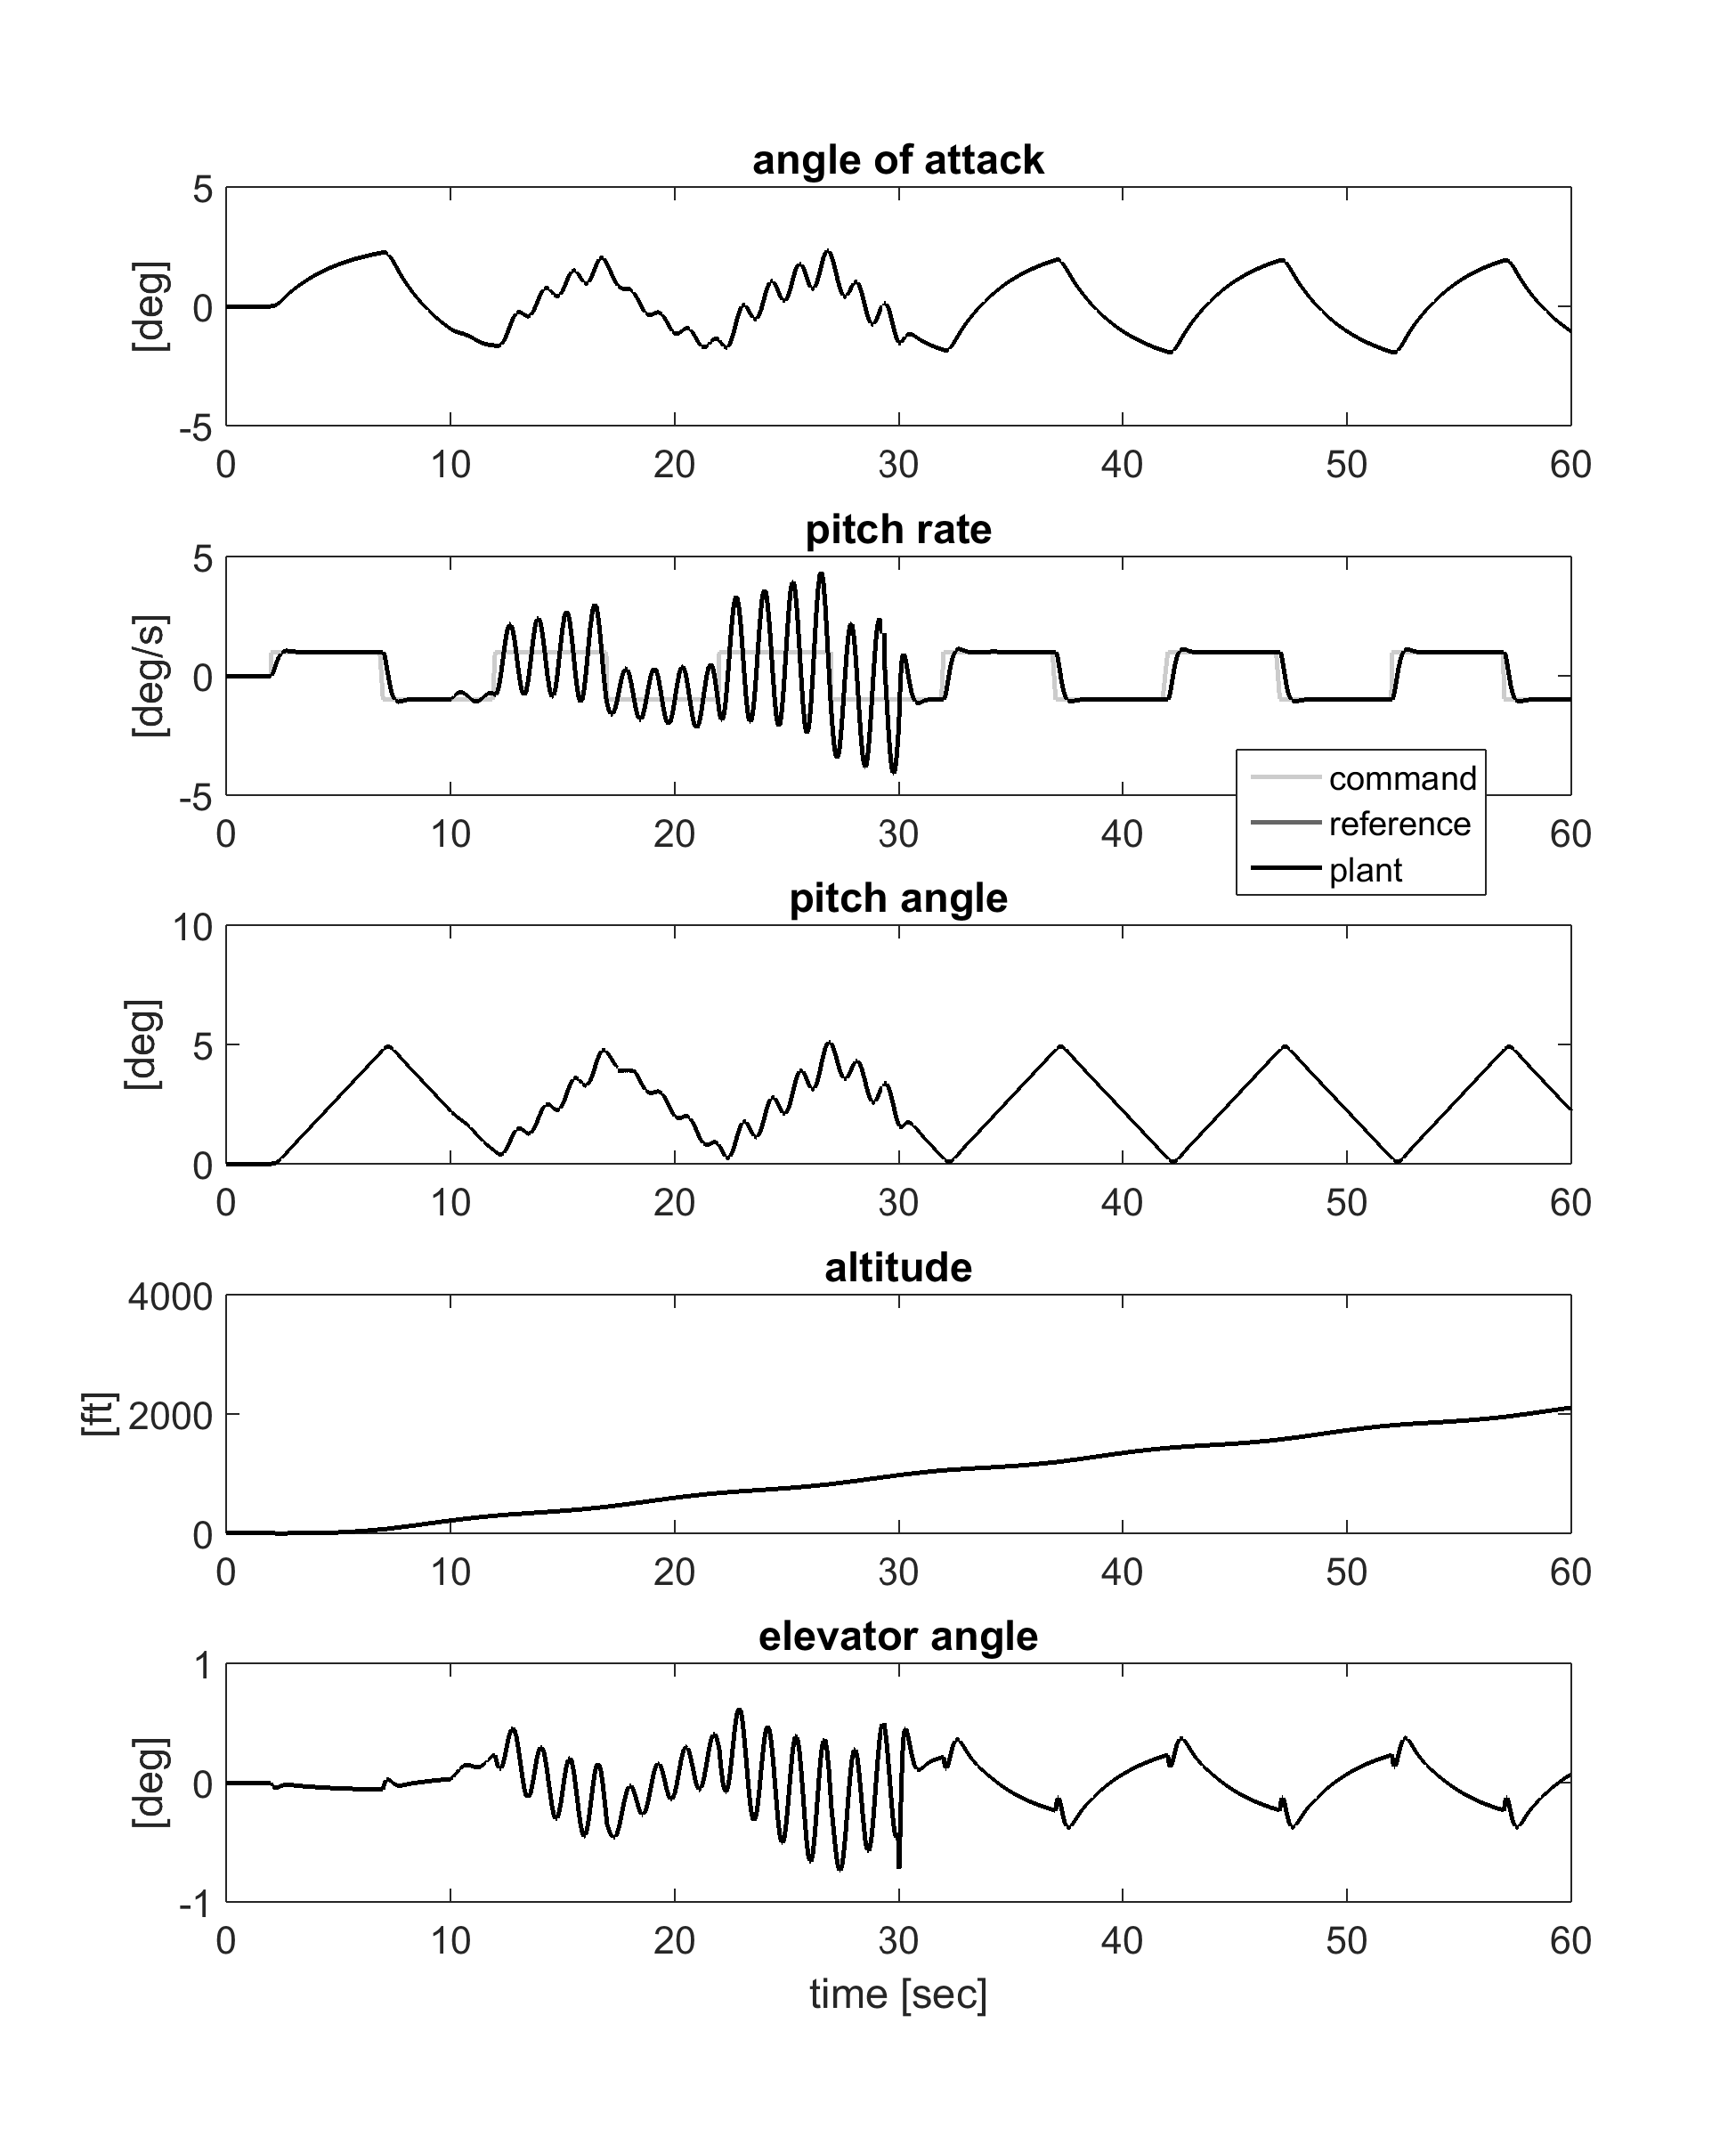
\includegraphics[width=6.5in]{\figurepath/innerLoopTransportLong.png}}
  \vspace{-0.95in}
  \caption{Time response of transport aircraft with inner-loop controller.\label{fig.innerLoopTransportLong}}
\end{figure}

\section{Conclusion}\label{sec.innerLoopConclusion}

This chapter presented a new alternative method for synthesizing a CRM based output feedback adaptive controller for a class of uncertain MIMO systems which do not have any unstable transmission zeros.
The controller is composed of a baseline control gain augmented with an adaptive component to accommodate control effectiveness uncertainty and matched plant uncertainty, and makes use of the closed-loop reference model to improve the transient properties of the overall adaptive system.
The adaptive controller requires the underlying error dynamics be made SPR through the synthesis of the postcompensator $S_{1}$ and CRM gain $L$.
The SPR relationship is enforced by reducing an underlying bilinear matrix inequality to a feasible linear matrix inequality through appropriate selection of a tuning matrix $X$.
The procedure does not require the plant first be squared-up.
It is computationally simple, and it requires only the calculation of some generalized inverses, the solution of the Lyapunov equation, and the solution of a reduced order state feedback problem.
This procedure is summarized in nine straightforward steps.
Furthermore, the degrees of freedom in the tuning matrix $X$ capture a large subset of all possible solutions which ensure the SPR property.
Using these degrees of freedom, $X$ can be tuned to provide the desired stability margins for the baseline system, as well as a globally stable update law.
The result is a baseline output feedback controller with good stability margins and adaptive augmentation capable of accommodating matched uncertainties.

This inner-loop design provided a controller capable of enforcing bounded reference tracking of $z_{p,\text{cmd}}(t)$ by $z_{p}(t)$, and accommodating uncertainties.
With the design of this inner-loop adaptive controller complete, the original control goal described in Chapter~\ref{ch.Introduction} has not yet been satisfied.
Recall that this control goal ultimately requires $u(t)$ in\ \eqref{eqn.wholeSystemUncertain} to be designed such that $z_{g}(t)$ tracks $z_{g,\text{cmd}}(t)$.
With the inner-loop designed providing $u(t)$ such that $z_{p}(t)$ tracks $z_{p,\text{cmd}}(t)$, the problem now becomes how to prescribe $z_{p,\text{cmd}}(t)$ such that $z_{g}(t)$ tracks $z_{g,\text{cmd}}(t)$.
The solution to this problem is described in Chapter~\ref{ch.outerLoop} which utilizes the existing inner-loop control design, but reintroduces the $B_{gd}$ term as in\ \eqref{eqn.innerLoopDynamicsUncertain} and considers the outer-loop dynamics in\ \eqref{eqn.outerLoopDynamics}.
